%\documentclass{article}
%
%% if you need to pass options to natbib, use, e.g.:
%%     \PassOptionsToPackage{numbers, compress}{natbib}
%% before loading neurips_2020
%
%% ready for submission
%% \usepackage{neurips_2020}
%
%% to compile a preprint version, e.g., for submission to arXiv, add add the
%% [preprint] option:
%\PassOptionsToPackage{numbers, compress}{natbib}
%% \usepackage[preprint]{neurips_2020}
%
%% to compile a camera-ready version, add the [final] option, e.g.:
%     \usepackage[final]{neurips_2020}
%
%% to avoid loading the natbib package, add option nonatbib:
%%     \usepackage[nonatbib]{neurips_2020}
%
%
%%\usepackage[utf8]{inputenc} % allow utf-8 input
%\usepackage[T1]{fontenc}    % use 8-bit T1 fonts
%\usepackage{hyperref}       % hyperlinks
%\usepackage{url}            % simple URL typesetting
%\usepackage{booktabs}       % professional-quality tables
%\usepackage{amsfonts}       % blackboard math symbols
%\usepackage{nicefrac}       % compact symbols for 1/2, etc.
%\usepackage{microtype}      % microtypography
%
%\usepackage{listings}
%\usepackage{graphicx}
%\usepackage{float}
%\usepackage{hyperref}
%\usepackage{graphicx}
%\usepackage{wrapfig}
%\usepackage{subfigure}
%\usepackage{booktabs}
%\usepackage{comment}
%\usepackage{amssymb}
%\usepackage{amsthm}
%\usepackage{amsmath}
%\usepackage{bm}
%\usepackage{dsfont}
%\usepackage{url}
%\usepackage{multirow}
%\usepackage{array}
%\usepackage{threeparttable}
%%\usepackage[ruled,linesnumbered]{algorithm2e}
%\usepackage[noend]{algpseudocode}
%\usepackage{color}
%%\usepackage[table]{xcolor}
%\usepackage{makecell}
%\usepackage{colortbl}
%\usepackage{rotating}
%\usepackage[normalem]{ulem}
%\DeclareMathOperator*{\argmin}{argmin}
%\usepackage{nomencl}
%\usepackage{bbm}
%\usepackage{marvosym}
%\usepackage{lipsum}
%\usepackage{caption}
%\usepackage{algorithm}
%\usepackage[noend]{algpseudocode}
%\usepackage{natbib}
%\usepackage[subtle]{savetrees} 
%
%% define code style
%\usepackage[dvipsnames]{xcolor}
%\definecolor{codegreen}{rgb}{0,0.6,0}
%\definecolor{codegray}{rgb}{0.5,0.5,0.5}
%\definecolor{codepurple}{rgb}{0.58,0,0.82}
%\definecolor{backcolour}{rgb}{0.95,0.95,0.92}
%\lstdefinestyle{mystyle}{
%    backgroundcolor=\color{backcolour},   
%    commentstyle=\color{codegreen},
%    keywordstyle=\color{magenta},
%    numberstyle=\tiny\color{codegray},
%    stringstyle=\color{codepurple},
%    basicstyle=\ttfamily\footnotesize,
%    breakatwhitespace=false,         
%    breaklines=true,                 
%    captionpos=b,                    
%    keepspaces=true,                 
%    numbers=left,                    
%    numbersep=5pt,                  
%    showspaces=false,                
%    showstringspaces=false,
%    showtabs=false,                  
%    tabsize=2
%}
%\lstset{style=mystyle}
%
%\newtheorem{theorem}{Theorem}
%\newtheorem{lemma}{Lemma}
%
%\makenomenclature
%\newcommand{\danny}[1]{\textcolor{blue}{DCA: #1}}
%\newcommand{\ryu}[1]{\textcolor{red}{#1}}
%\newcommand{\lezhang}[1]{\textcolor{orange}{#1}}
%\newcommand{\etal}{\textit{et al.}}

\chapter{Modelling Human Uncertainty (II): Segmentation} \label{chapter:humanuncertainty_seg}
%\title{Neural Fusion Network for Segmentation of Uncertainty Images}

% The \author macro works with any number of authors. There are two commands
% used to separate the names and addresses of multiple authors: \And and \AND.
%
% Using \And between authors leaves it to LaTeX to determine where to break the
% lines. Using \AND forces a line break at that point. So, if LaTeX puts 3 of 4
% authors names on the first line, and the last on the second line, try using
% \AND instead of \And before the third author name.

  % examples of more authors
  % \And
  % Coauthor \\
  % Affiliation \\
  % Address \\
  % \texttt{email} \\
  % \AND
  % Coauthor \\
  % Affiliation \\
  % Address \\
  % \texttt{email} \\
  % \And
  % Coauthor \\
  % Affiliation \\
  % Address \\
  % \texttt{email} \\
  % \And
  % Coauthor \\
  % Affiliation \\
  % Address \\
  % \texttt{email} \\


\paragraph{Abstract: }
In this chapter, we extend the method introduced in Chapter~\ref{chapter:humanuncertainty} to the more challenging task of semantic segmentation where every pixel in a given input image is classified. To this end, we model the annotation mistakes of each annotator as a pixel-wise confusion matrix that is a function of the input image. Analogous to the classification approach, the separation between the true labels and the annotation mistakes is achieved by encouraging the estimated annotators to be maximally unreliable while achieving high fidelity with the noisy training data. We first define a toy segmentation dataset based on the MNIST dataset and empirically study the behaviours of the proposed algorithm. We then demonstrate the utility of the method on three public medical imaging segmentation datasets with simulated (when necessary) and real diverse annotations: 1) MSLSC (multiple-sclerosis lesions); 2) BraTS (brain tumours); 3) LIDC-IDRI (lung abnormalities). In all cases, our method outperforms competing methods and relevant baselines particularly in cases where the number of annotations is small and the amount of disagreement is large. The experiments also show strong ability to capture the complex spatial characteristics of annotators' mistakes. Our code is available at \url{https://github.com/moucheng2017/Learn_Noisy_Labels_Medical_Images}. This chapter is based on a joint work \cite{zhang2020disentangling} with Le Zhang at UCL. 

%\renewcommand{\thefootnote}{}
%\footnotetext{*These authors contributed equally.}

\section{Introduction}

% \ryu{(Ryu): ``I would probably introduce the issue of inter-reader variation more broadly in the context of medical imaging applications, and then narrow our focus on the segmentation problem. For example, we can certainly highlight that many vision applications in medical image analysis \cite{litjens2017survey} require annotations from clinical experts, which incur high costs and commonly suffer from high inter-reader variability \cite{watadani2013interobserver,rosenkrantz2013comparison,lazarus2006bi,warfield2004simultaneous}. Also, another piece of evidence within the segmentation context that we can refer to alongside the MS lesion example:  the average variability in the range 74-85\% has been reported for glioblastoma segmentation \cite{menze2014multimodal}.'' }


Segmentation of anatomical structures in medical images is known to suffer from high inter-reader variability \cite{lazarus2006bi,watadani2013interobserver,rosenkrantz2013comparison,menze2014multimodal,joskowicz2019inter}, influencing the performance of downstream supervised machine learning models. This problem is particularly prominent in the medical domain where the labelled data is commonly scarce due to the high cost of annotations. For instance, accurate identification of multiple sclerosis (MS) lesions in MRIs is difficult even for experienced experts due to variability in lesion location, size, shape and anatomical variability across patients \cite{zhang2019multiple}. Another example \cite{menze2014multimodal} reports the average inter-reader variability in the range 74-85\% for glioblastoma (a type of brain tumour) segmentation. Further aggravated by differences in biases and levels of expertise, segmentation annotations of structures in medical images suffer from high annotation variations \cite{kats2019soft}. In consequence, despite the present abundance of medical imaging data thanks to over two decades of digitisation, the world still remains relatively short of access to data with curated labels \cite{harvey2019standardised}, that is amenable to machine learning, necessitating intelligent methods to learn robustly from such noisy annotations.

To mitigate inter-reader variations, different pre-processing techniques are commonly used to curate segmentation annotations by fusing labels from different experts. The most basic yet popular approach is based on the majority vote where the most representative opinion of the experts is treated as the ground truth (GT). A smarter version that accounts for similarity of classes has proven effective in aggregation of brain tumour segmentation labels \cite{menze2014multimodal}. A key limitation of such approaches, however, is that all experts are assumed to be equally reliable. Warfield \etal \cite{warfield2004simultaneous} proposed a label fusion method, called STAPLE that explicitly models the reliability of individual experts and uses that information to ``weigh'' their opinions in the label aggregation step. After consistent demonstration of its superiority over the standard majority-vote pre-processing in multiple applications, STAPLE has become the go-to label fusion method in the creation of public medical image segmentation datasets e.g., ISLES \cite{winzeck2018isles}, MSSeg \cite{commowick2018objective}, Gleason'19 \cite{gleason2019} datasets. Asman \etal later extended this approach in \cite{asman2011robust} by accounting for voxel-wise consensus to address the issue of under-estimation of annotators' reliability. In \cite{asman2012formulating}, another extension was proposed in order to model the reliability of annotators across different pixels in images. More recently, within the context of multi-atlas segmentation problems \cite{iglesias2013unified} where image registration is used to warp segments from labeled images (``atlases'') onto a new scan, STAPLE has been enhanced in multiple ways to encode the information of the underlying images into the label aggregation process. A notable example is STEP proposed in Cardoso \etal \cite{cardoso2013steps} who designed a strategy to further incorporate the local morphological similarity between atlases and target images, and different extensions of this approach such as \cite{asman2013non,akhondi2014logarithmic} have since been considered. However, these previous label fusion approaches have a common drawback---they critically lack a mechanism to integrate information across different training images. This fundamentally limits the remit of applications to cases where each image comes with a reasonable number of annotations from multiple experts, which can be prohibitively expensive in practice. Moreover, relatively simplistic functions are used to model the relationship between observed noisy annotations, true labels and reliability of experts, which may fail to capture complex characteristics of human annotators.


% However, all these intensity-based approaches assume that a set of atlases i.e., ``training examples'' with clean labels are available. 

% \danny{Generally avoid starting paragraphs with "however" - means that the sentence refers to the previous sentence, so almost always should be in the same paragraph. Here it's particularly unclear what the 'however' refers to as the previous sentence also begins with a 'however'. Thoughts need reorganising.}




% % Biomedical image anatomical segmentation is a fundamental problem in medical image analysis.

% Image segmentation tasks assign a class label to each pixel in an image. In many cases the context in the image provides sufficient information to resolve the ambiguities during this mapping. However, there exists a special class of images where even the complete image context isn't sufficient to resolve all ambiguities. Such ambiguities are common in medical imaging applications, e.g., in multiple sclerosis (MS) lesions segmentation from brain MRI images. A lesion could be clearly visible, but the knowledge about whether it's lesion tissue or not won't be available from this image alone. Thus, accurate identification of multiple sclerosis (MS) lesions in MRIs is difficult even for experienced experts due to variability in lesion location, size, shape and anatomical variability across patients \cite{zhang2019multiple}.


% % \ryu{(Ryu): ``I would rethink whether to move the following to related work --- perhaps better to keep our focus on the healthcare relevance, although it may benefit to briefly mention the wider prevalence of the problem outside medical imaging ...'': } 
% % Similar ambiguities also are present in photos. E.g. a Canada goose might be easily recognized by bird experts, but it's difficult for the non-experts, which could consider it as a black-neck duck or just a bird. Most existing segmentation algorithms either provide just one likely consistent hypothesis (e.g., “all pixels belong to a Canada goose”) or a pixel-wise probability (e.g., “each pixel is 50\% Canada goose and 50\% black-neck duck”). 

% In medical applications where a subsequent diagnosis or a treatment depends on the segmentation map, annotations of MS lesions suffer from high annotation variations because of the further aggravated by differences in levels of expertise \cite{kats2019soft}. Traditional machine learning algorithms trained on annotation with uncertainty provide only pixel-wise probabilities ignores all co-variances between the pixels, which makes a subsequent analysis far more difficult if not impossible. Despite the present abundance of medical imaging data thanks to over two decades of digitisation, the world still remains relatively short of access to data with curated labels \cite{harvey2019standardised}, that is amenable to machine learning, necessitating an intelligent method to learn robustly from such noisy annotations.

%Especially in medical applications where a subsequent diagnosis or a treatment depends on the segmentation map, an algorithm that only provides the foremost likely hypothesis might cause misdiagnoses and sub-optimal treatment. Providing only pixel-wise probabilities ignores all co-variances between the pixels, which makes a subsequent analysis far more difficult if not impossible. If multiple consistent hypotheses are provided, these are often directly propagated into subsequent step during a diagnosis pipeline, they will be wont to suggest further diagnostic tests to resolve the ambiguities, or an expert with access to additional information can select the acceptable one(s) for the next steps.

% \ryu{(Ryu): ``We have to justify the need for developing a new framework --- we have to mention the relevant prior work and argue that they are not sufficient as we have done in our MICCAI submission (e.g., STAPLE-based label aggregation methods), but perhaps in a wider context. We know that the STAPLE variants are not good enough. We can also mention more generic approaches to learning from noisy labels but these methods are typically only designed for classification, and thus these are not enough either. So, we needed to develop our own solution ... (lead to the next paragraph) ''}


In this work, we introduce the first instance of an end-to-end supervised segmentation method that jointly estimates, from noisy labels alone, the reliability of multiple human annotators and true segmentation labels. The proposed architecture (Fig.~\ref{picture 2}) consists of two coupled CNNs where one estimates the true segmentation probabilities and the other models the characteristics of individual annotators (e.g., tendency to over-segmentation, mix-up between different classes, etc) by estimating the pixel-wise confusion matrices (CMs) on a per image basis. Unlike STAPLE \cite{warfield2004simultaneous} and its variants, our method models, and disentangles with deep neural networks, the complex mappings from the input images to the annotator behaviours and to the true segmentation label. Furthermore, the parameters of the CNNs are ``global variables'' that are optimised across different image samples; this enables the model to disentangle robustly the annotators' mistakes and the true labels based on correlations between similar image samples, even when the number of available annotations is small per image (e.g., a single annotation per image). In contrast, this would not be possible with STAPLE \cite{warfield2004simultaneous} and its variants \cite{asman2012formulating,cardoso2013steps} where the annotators' parameters are estimated on every target image separately.

% \danny{Not sure what you mean by "global variables"; do you independent of individual images? Need to specify more precisely I think.} and 

% extend STAPLE \cite{warfield2004simultaneous} \danny{further to comment in the abstract, I would not say it like this as it sounds incremental. Try something like "Unlike STAPLE, our method..." or "While STAPLE ... does something, our method ... does something better} to the supervised learning setting, and introduce a method for jointly estimating the reliability of multiple annotators and true segmentation label via deep neural networks. 

For evaluation, we first simulate a diverse range of annotator types on the MNIST dataset by performing morphometric operations with Morpho-MNIST framework \cite{castro2019morphomnist}. Then we demonstrate the potential in several real-world medical imaging datasets, namely (i) MS lesion segmentation dataset (MSLSC) from the ISBI 2015 challenge \cite{styner20083d}, (ii) Brain tumour segmentation dataset (BraTS) \cite{menze2014multimodal} and (iii) Lung nodule segmentation dataset (LIDC-IDRI) \cite{armato2011lung}. Experiments on all datasets demonstrate that our method consistently leads to better segmentation performance compared to widely adopted label-fusion methods and other relevant baselines, especially when the number of available labels for each image is low and the degree of annotator disagreement is high. 
% We also show that our model is capable of recovering the true label distributions even when there is only one label available per example. 

% Here we present a segmentation framework that provides multiple segmentation annotators for ambiguous images \danny{sentence doesn't make sense - what do you mean it "provides multiple ... annotators"?  It outputs humans??}. Our framework extends \danny{further to comment in the abstract, I would not say it like this as it sounds incremental. Try something like "Unlike STAPLE, our method..." or "While STAPLE ... does something, our method ... does something better} STAPLE (Simultaneous Truth and Performance Level Estimation), which can jointly estimate the reliability of multiple annotators and true segmentation label via deep neural networks. The proposed architecture consists of two coupled CNNs where one estimates the true segmentation probabilities and the other models the characteristics of individual annotators (e.g., prone to over-segmentation) by estimating pixel-wise confusion matrices on a per image basis \danny{Are confusion matrices per image or per annotator? If they are characteristics of teh annotator as you suggest, then surely the latter}. The parameters of our models are global variables and optimised across different image samples; this enables the model to infer annotators’ characteristics and true labels based on correlations between similar image samples even when only a single annotation is available per image. In contrast, this would not be possible with STAPLE \cite{warfield2004simultaneous} and its variants \cite{asman2012formulating,cardoso2013steps} where the annotators’ parameters are estimated on every image separately.


\section{Related Work}
\vspace{-2mm}

The majority of algorithmic innovations in the space of \textit{label aggregation for segmentation} have uniquely originated from the medical imaging community, partly due to the prominence of the inter-reader variability problem in the field, and the wide-reaching values of reliable segmentation methods \cite{asman2012formulating}. The aforementioned methods based on the STAPLE-framework such as \cite{warfield2004simultaneous,asman2011robust,asman2012formulating,cardoso2013steps,weisenfeld2011learning,asman2013non,asman2013non,akhondi2014logarithmic,joskowicz2018automatic} are based on generative models of human behaviours, where the latent variables of interest are the unobserved true labels and the ``reliability'' of the respective annotators. Our method can be viewed as an instance of translation of the STAPLE-framework to the supervised learning paradigm. As such, our method produces a model that can segment test images without needing to acquire labels from annotators or atlases unlike STAPLE and its local variants. Another key difference is that our method is jointly trained on many different subjects while the STAPLE-variants are only fitted on a per-subject basis. This means that our method is able to learn from correlations between different subjects, which previous works have not attempted--- for example, our method uniquely can estimate the reliability and true labels even when there is only one label available per input image as shown later. 

Our work also relates to a recent strand of methods that aim to generate a set of diverse and plausible segmentation proposals on a given image. Notably, probabilistic U-net \cite{kohl2018probabilistic} and its recent variants, PHiSeg \cite{baumgartner2019phiseg} have shown that the aforementioned inter-reader variations in segmentation labels can be modelled with sophisticated forms of probabilistic CNNs. Such approaches, however, fundamentally differ from ours in that variable annotations from many experts in the training data are assumed to be all realistic instances of the true segmentation; we assume, on the other hand, that there is a single, unknown, true segmentation map of the underlying anatomy, and each individual annotator produces a noisy approximation to it with variations that reflect their individual characteristics. The latter assumption may be reasonable in the context of segmentation problems since there exists only one true boundary of the physical objects captured in an image while multiple hypothesis can arise from ambiguities in human interpretations.

% \ryu{(Ryu); How about weakly supervised segmentation method e.g., learning from scribbles, etc} 

We also note that, in standard classification problems, a plethora of different works have shown the utility of modelling the labeling process of human annotators in restoring the true label distribution \cite{raykar2010learning,khetan2017learning,tanno2019learning}. Such approaches can be categorized into two groups: (1) \textit{two-stage} approach \cite{dawid1979maximum,smyth1995inferring,whitehill2009whose,welinder2010multidimensional,rodrigues2013learning}, and (2) \textit{simultaneous} approach \cite{raykar2009supervised,yan2010modeling,branson2017lean,van2018lean,khetan2017learning,tanno2019learning,sudre2019let}. In the first category, the noisy labels are first curated through a probabilistic model of annotators, and subsequently, a supervised machine-learning model is trained on the curated labels. The initial attempt \cite{dawid1979maximum} was made in the early 1970s, and numerous advances such as \cite{smyth1995inferring,whitehill2009whose,welinder2010multidimensional,rodrigues2013learning} since built upon this work e.g. by estimating sample difficulty and human biases. In contrast, models in the second category aim to curate labels and learn a supervised model jointly in an end-to-end fashion \cite{raykar2009supervised,yan2010modeling,branson2017lean,van2018lean,khetan2017learning,tanno2019learning} so that the two components inform each other. Although the evidence still remains limited to the simple classification task, these \textit{simultaneous} approaches have shown promising improvements over the methods in the first category in terms of the predictive performance of the supervised model and the sample efficiency (i.e., fewer labels are required per input). However, to date very little attention has been paid to the same problem in more complicated, structured prediction tasks where the outputs are high dimensional. In this work, we propose the first \textit{simultaneous} approach to addressing such a problem for image segmentation, while drawing inspirations from the STAPLE framework \cite{warfield2004simultaneous} which would fall into the \textit{two-stage} approach category. 


% Previous work proposed various methods for jointly estimating the skills of the annotators and the ground truth (GT) labels. We categorize these methods into two groups: (1) \textit{two-stage} approach and (2) \textit{simultaneous} approach. Methods in the first category perform label aggregation and training of a supervised learning model in two separate steps. The noisy labels $\widetilde{\mathbf{Y}}$ are first aggregated by building a probabilistic model of annotators. The observable variables are the noisy labels $\widetilde{\mathbf{Y}}$, and the latent variables/parameters to be estimated are the annotator skills and GT labels $\mathbf{Y}$. Then, a machine learning model is trained on the pairs of aggregated labels $\mathbf{Y}$ and input examples $\mathbf{X}$ (e.g. images) to perform the task of interest. The initial attempt was made in \cite{dawid1979maximum} in the early 1970s and more recently, numerous lines of research \cite{smyth1995inferring,warfield2004simultaneous,whitehill2009whose,welinder2010multidimensional,rodrigues2013learning} proposed extensions of this work e.g. by estimating the difficulty of each example. However, in all these cases, information about the raw inputs $\mathbf{X}$ is completely neglected in the generative model of noisy labels used in the aggregation step, and this highly limits the quality of estimated true labels in practice.

% The \textit{simultaneous} approaches \cite{raykar2009supervised,yan2010modeling,branson2017lean,van2018lean} address this issue by integrating the prediction of the supervised learning model (i.e. distribution $p(\mathbf{Y}|\mathbf{X})$) into the probabilistic model of noisy labels, and have been shown to improve the predictive performance. These methods employ variants of the expectation-maximization (EM) algorithm during training, and require a reasonable number of labels for each example. However, in most real world applications, it is practically prohibitive to collect a large number of labels per example, and this requirement limits their applications. A notable exception is the Model Boostrapped EM (MBEM) algorithm presented in \cite{khetan2017learning} that is capable of learning even with little label redundancy. 


% \ryu{(Ryu): Expand on the following - the categorisation of two-stage and simultaneous approaches from \cite{tanno2019learning} would be useful.}


% See the paragraphs below: 

% However, if the exact process by which each annotator generates the labels was known, we could correct the annotations accordingly and thus train our model on a cleaner set of data. Furthermore, this additional knowledge of the annotators' skills can be utilized to decide on which examples to be labeled by which annotators \cite{welinder2010online,long2013active,long2015multi}. Therefore, methods that can accurately model the label noise of annotators are useful for improving not only the accuracy of the trained model, but also the quality of labels in the future. 

% Previous work proposed various methods for jointly estimating the skills of the annotators and the ground truth (GT) labels. We categorize these methods into two groups: (1) \textit{two-stage} approach and (2) \textit{simultaneous} approach. Methods in the first category perform label aggregation and training of a supervised learning model in two separate steps. The noisy labels $\widetilde{\mathbf{Y}}$ are first aggregated by building a probabilistic model of annotators. The observable variables are the noisy labels $\widetilde{\mathbf{Y}}$, and the latent variables/parameters to be estimated are the annotator skills and GT labels $\mathbf{Y}$. Then, a machine learning model is trained on the pairs of aggregated labels $\mathbf{Y}$ and input examples $\mathbf{X}$ (e.g. images) to perform the task of interest. The initial attempt was made in \cite{dawid1979maximum} in the early 1970s and more recently, numerous lines of research \cite{smyth1995inferring,warfield2004simultaneous,whitehill2009whose,welinder2010multidimensional,rodrigues2013learning} proposed extensions of this work e.g. by estimating the difficulty of each example. However, in all these cases, information about the raw inputs $\mathbf{X}$ is completely neglected in the generative model of noisy labels used in the aggregation step, and this highly limits the quality of estimated true labels in practice.

% The \textit{simultaneous} approaches \cite{raykar2009supervised,yan2010modeling,branson2017lean,van2018lean} address this issue by integrating the prediction of the supervised learning model (i.e. distribution $p(\mathbf{Y}|\mathbf{X})$) into the probabilistic model of noisy labels, and have been shown to improve the predictive performance. These methods employ variants of the expectation-maximization (EM) algorithm during training, and require a reasonable number of labels for each example. However, in most real world applications, it is practically prohibitive to collect a large number of labels per example, and this requirement limits their applications. A notable exception is the Model Boostrapped EM (MBEM) algorithm presented in \cite{khetan2017learning} that is capable of learning even with little label redundancy. 

% More broadly, our work is related to methods for robust learning in the presence of label noise. There is a large body of literature that do not explicitly model individual annotators unlike our method. 

% %Natarajan et al. \cite{natarajan2013learning} proposed a generic unbiased estimator of any loss function for binary classification with noisy labels and gave theoretical bounds on the performance.
% The effects of label noise are well studied in common classifiers such as SVMs and logistic regression, and robust variants have been proposed \cite{frenay2014classification,natarajan2013learning,bootkrajang2012label}.  More recently, various attempts have been made to train deep neural networks under label noise.  Reed et al. \cite{reed2014training} developed a robust loss to model ``prediction consistency", which was later extended by \cite{tanaka2018joint}. %with an extra procedure to replace the original noisy labels with the model predictions.
% In \cite{mnih2012learning} and \cite{sukhbaatar2014training}, label noise was parametrized in the form of a transition matrix and incorporated into neural networks for binary and multi-way classification. A more effective alternative for estimating such transition matrix was proposed in \cite{patrini2017making}, and a method for capturing image dependency of label noise was shown in \cite{Goldberger2017TrainingDN}. We will later compare our model to several of these methods to test the value of modelling individual annotators in gaining robustness to label noise. 

% Multiple lines of work have shown that a small portion of clean labels improves robustness. \cite{veit2017learning} proposed to learn from clean labels to correct the labels of noisy examples. \cite{ren2018learning} proposed a method for learning to weigh examples during each training iteration by using the validation loss on clean labels as the meta-objective. \cite{jiang2018mentornet} employs a similar approach, but trains a separate network that proposes weighting. However, curating a set of clean labels of sufficient size is expensive for many applications, and this work focuses on the scenario of learning from purely noisy labels. 


\begin{figure}[t]
    \centering
    \vspace{-2mm}
    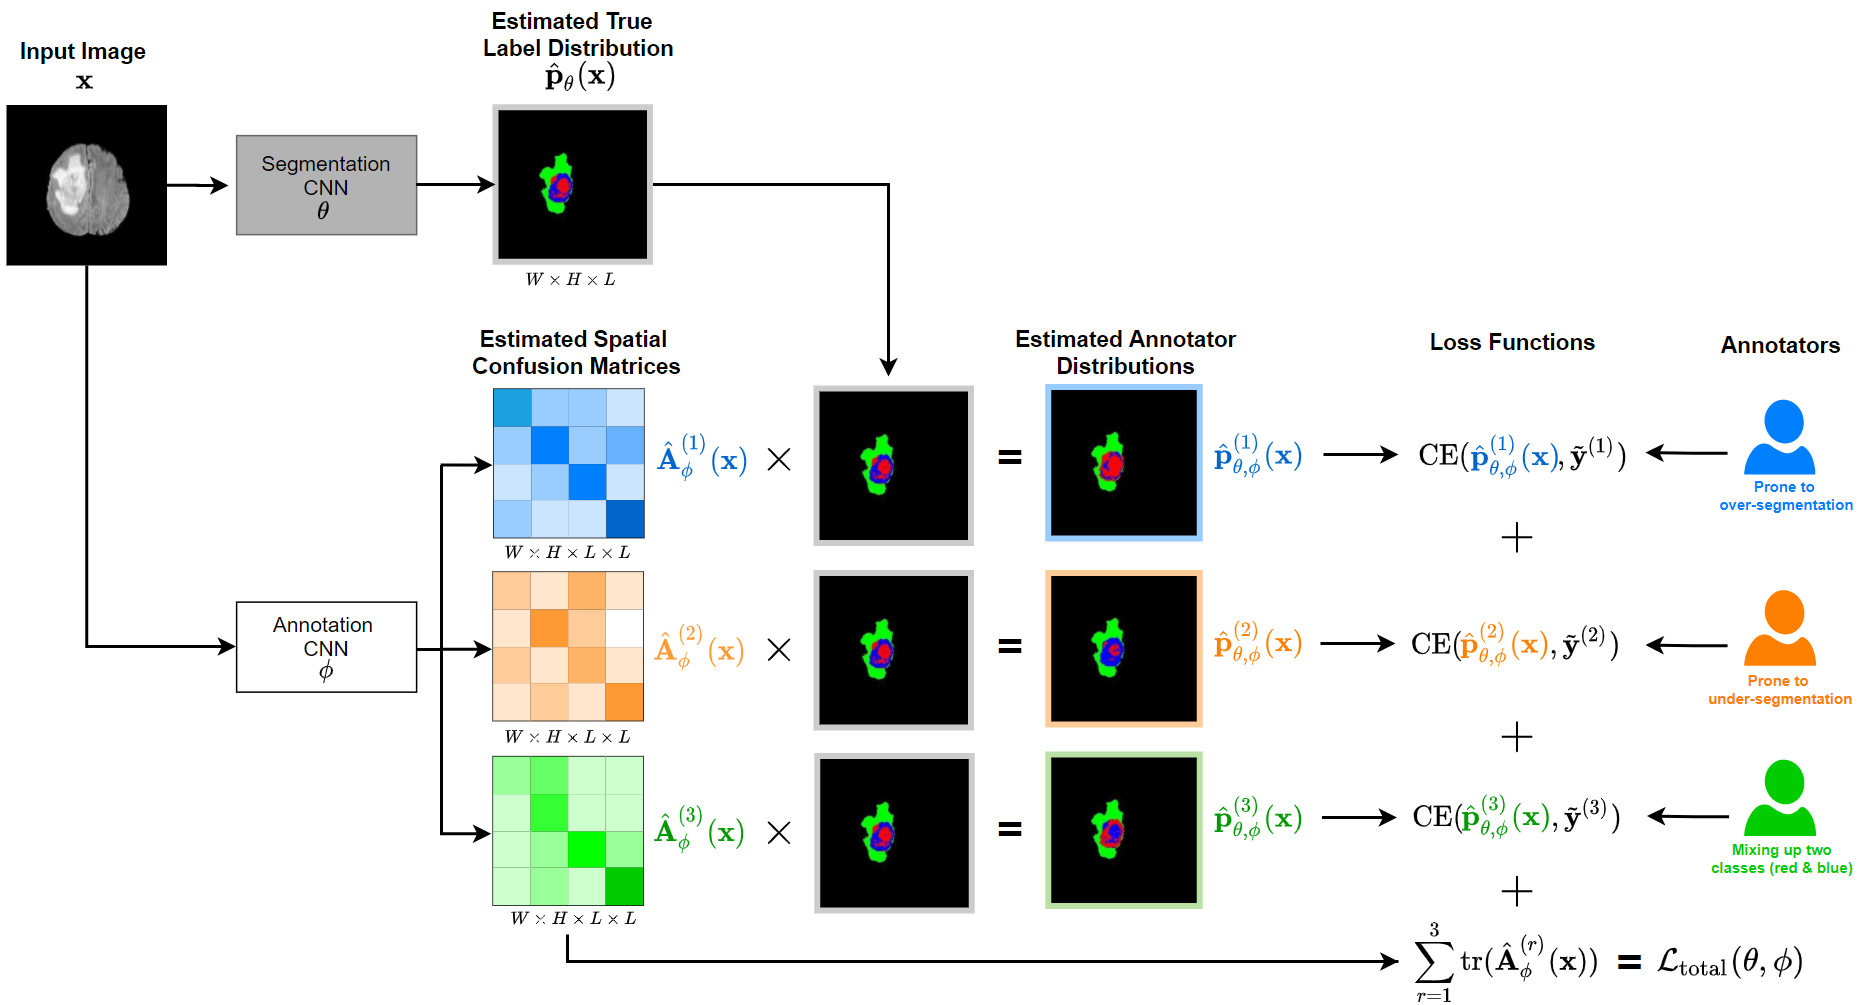
\includegraphics[width=\linewidth]{chapter_8_neurips/picture22.png}
    \caption{\footnotesize An architecture schematic in the presence of 3 annotators of varying characteristics (over-segmentation, under-segmentation and confusing between two classes, red and blue). The model consists of two parts: (1) \textit{segmentation network} parametrised by $\theta$ that generates an estimate of the unobserved true segmentation probabilities, $\textbf{p}_{\theta}(\textbf{x})$; (2) \textit{annotator network}, parametrised by $\phi$, that estimates the pixelwise confusion matrices (CMs), $\{\textbf{A}_{\phi}^{(r)}(\textbf{x})\}_{r=1}^{3}$ of the annotators  for the given input image $\textbf{x}$. During training, the estimated annotators distributions $\hat{\textbf{p}}_{\theta,\phi}^{(r)}(\textbf{x}):=\textbf{A}_{\phi}^{(r)}(\textbf{x})\cdot\textbf{p}_{\theta}(\textbf{x})$ are computed, and the parameters $\{\theta, \phi\}$ are learned by minimizing the sum of their cross-entropy losses with respect to the acquired noisy segmentation labels $\tilde{\mathbf{y}}^{(r)}$, and the trace of the estimated CMs. At test time, the output of the segmentation network, $\hat{\textbf{p}}_{\theta}(\textbf{x})$ is used to yield the prediction.}
    %The segmentation probabilities of respective annotators $\hat{\textbf{p}}_{\phi}^{(r)}(\textbf{x}):=\textbf{A}_{\phi}^{(r)}(\textbf{x})\cdot\textbf{p}_{\theta}(\textbf{x})$ are then computed. The model parameters $\{\theta, \phi\}$ are optimized to minimize the sum of five cross-entropy losses between each estimated annotator distribution $\textbf{p}_{\phi}^{(r)}(\textbf{x})$ and the noisy labels $\tilde{\textbf{y}}^{(r)}$ observed from each annotator.} 
    \label{picture 2}
\end{figure}


\section{Method}
\vspace{-2mm}

% \ryu{(RYU): Write a short background section to contrast with the prior approaches to aggregating labels, and how our approaches differ from them. If short of space, move to supp materials and leave a pointer. The key differences to highlight are the translations of these framework to the supervised learning setting \& can learn from correlations between different images. } 

% \ryu{(RYU): Another thing is the extension of the main theorem in Tanno et al., CVPR'19 \cite{tanno2019learning} to the segmentation problem. State it and explain it, but leave the proof in the supplementary. } 

% \danny{Not read in detail}

\subsection{Problem Set-up}
\vspace{-2mm}

In this work, we consider the problem of learning a supervised segmentation model from noisy labels acquired from multiple human annotators. Specifically, we consider a scenario where set of images $\{\textbf{x}_n \in \mathbb{R}^{W\times H\times C}\}_{n=1}^N$ (with $W, H, C$ denoting the width, height and channels of the image) are assigned with noisy segmentation labels $\{\tilde{\textbf{y}}_n^{(r)} \in \mathcal{Y}^{W\times H}\}_{n=1,...,N}^{r\in S(\mathbf{x}_i)}$ from multiple annotators where $\tilde{\textbf{y}}_n^{(r)}$ denotes the label from annotator $r \in \{1,...,R\}$ and $S(\mathbf{x}_n)$ denotes the set of all annotators who labelled image $\textbf{x}_i$ and $\mathcal{Y}=[1, 2,...,L]$ denotes the set of classes. 

Here we assume that every image $\mathbf{x}$ annotated by at least one person i.e., $|S(\mathbf{x})|\geq 1$, and no GT labels $\{\textbf{y}_n \in \mathcal{Y}^{W\times H} \}_{n=1,...,N}$ are available. The problem of interest here is to \textit{learn the unobserved true segmentation distribution $p(\textbf{y} \mid \textbf{x})$ from such noisy labelled dataset $\mathcal{D}=\{\textbf{x}_n, \tilde{\textbf{y}}_n^{(r)}\}^{r\in S(\mathbf{x}_n)}_{n=1,...,N}$} i.e., the combination of images, noisy annotations and experts' identities for labels (which label was obtained from whom). 

We also emphasise that \textit{the goal at inference time is to segment a given unlabelled test image} but not to fuse multiple available labels as is typically done in multi-atlas segmentation approaches \cite{iglesias2013unified}. 

\vspace{-2mm}
\subsection{Probabilistic Model and Proposed Architecture}
Here we describe the probabilistic model of the observed noisy labels from multiple annotators. We make two key assumptions: (1) annotators are statistically independent, (2) annotations over different pixels are independent given the input image. Under these assumptions, the probability of observing noisy labels $\{\tilde{\textbf{y}}^{(r)}\}_{r\in S(\mathbf{x})}$ on $\textbf{x}$ factorises as:
\begin{equation}
    p(\{\tilde{\textbf{y}}^{(r)}\}_{r\in S(\mathbf{x})}\mid \textbf{x})
    =\prod_{r\in S(\mathbf{x})}p(\tilde{\textbf{y}}^{(r)}\mid \textbf{x})
    = \prod_{r\in S(\mathbf{x})}\prod_{\substack{w\in\{1,...,W\}\\h\in\{1,...,H\}}} p(\tilde{y}^{(r)}_{wh} \mid \textbf{x})
    \label{eq:joint_probs}
\end{equation}
where $\tilde{y}^{(r)}_{wh} \in [1, ..., L]$ denotes the $(w, h)^{\text{th}}$ elements of $\tilde{\textbf{y}}^{(r)}\in \mathcal{Y}^{W\times H}$. Now we rewrite the probability of observing each noisy label on each pixel $(w, h)$ as: 
\begin{equation}
    p(\tilde{y}^{(r)}_{wh}\mid \textbf{x})= \sum_{y_{wh}= 1}^{L} p(\tilde{y}^{(r)}_{wh}\mid y_{wh},\textbf{x}) \cdot  p(y_{wh}\mid \textbf{x}) 
    \label{eq:confusion_matrix}
\end{equation}
where $p(y_{wh}\mid\textbf{x})$ denotes the GT label distribution over the $(w, h)^{\text{th}}$ pixel in the image $\textbf{x}$, and $p(\tilde{y}^{(r)}_{wh}\mid y_{wh},\textbf{x})$ describes the noisy labelling process by which annotator $r$ corrupts the true segmentation label. In particular, we refer to the $L\times L$ matrix whose each $(i,j)^{\text{th}}$ element is defined by the second term $\textbf{a}^{(r)}(\mathbf{x},w,h)_{ij}:=p(\tilde{y}^{(r)}_{wh}=i\mid y_{wh}=j,\textbf{x})$ as the CM of annotator $r$ at pixel $(w, h)$ in image $\mathbf{x}$. 

We introduce a CNN-based architecture which models the different constituents in the above joint probability distribution $p(\{\tilde{\textbf{y}}^{(r)}\}_{r\in S(\mathbf{x})}\mid \textbf{x})$ as illustrated in Fig. \ref{picture 2}. The model consists of two components: (1) \textit{Segmentation Network}, parametrised by $\theta$, which estimates the GT segmentation probability map, $\hat{\textbf{p}}_{\theta}(\textbf{x}) \in \mathbb{R}^{W\times H \times L}$ whose each $(w, h, i)^\text{th}$ element approximates $p(y_{wh}=i\mid \textbf{x})$;(2) \textit{Annotator Network}, parametrised by $\phi$, that generate estimates of the pixel-wise CMs of respective annotators as a function of the input image, $\{\hat{\textbf{A}}_{\phi}^{(r)}(\textbf{x})\in [0,1]^{W\times H\times L \times L}\}_{r=1}^{R}$ whose each $(w, h, i, j)^\text{th}$ element approximates $p(\tilde{y}^{(r)}_{wh}=i\mid y_{wh}=j,\textbf{x})$. Each product ${\hat{\textbf{p}}_{\theta, \phi}^{(r)}}(\textbf{x}):=\hat{\textbf{A}}_{\phi}^{(r)}(\textbf{x})\cdot \hat{\textbf{p}}_\theta (\textbf{x})$ represents the estimated segmentation probability map of the corresponding annotator. Note that here ``$\,\cdot\,$'' denotes the element-wise matrix multiplications in the spatial dimensions $W, H$. At inference time, we use the output of the segmentation network ${\hat{\textbf{p}}_\theta }(\textbf{x})$ to segment test images. 

We note that each spatial CM, $\hat{\textbf{A}}_{\phi}^{(r)}(\textbf{x})$ contains $WHL^2$ variables, 
and calculating the corresponding annotator's prediction $\hat{\textbf{p}}_{\theta, \phi}^{(r)}(\textbf{x})$ requires $WH(2L-1)L$ floating-point operations, potentially incurring a large time/space cost when the number of classes is large. Although not the focus of this work (as we are concerned with medical imaging applications for which the number of classes are mostly limited to less than 10), we also consider a low-rank approximation (rank$=1$) scheme to alleviate this issue wherever appropriate. More details are provided in the supplementary.

\subsection{Learning Confusion Matrices and True Segmentation}

Next, we describe how we jointly optimise the parameters of segmentation network, $\theta$ and the parameters of annotator network, $\phi$. In short, we minimise the negative log-likelihood of the probabilistic model plus a regularisation term via stochastic gradient descent. A detailed description is provided below. 

Given training input $\textbf{X}=\{\textbf{x}_n\}_{n=1}^N$ and noisy labels ${\tilde{\textbf{Y}}^{(r)}} = \{ \tilde{ \textbf{y}}_n^{(r)}: r \in S(\textbf{x}_n)\} _{n = 1}^N$ for $r=1,...,R$, we optimaize the parameters $\{ \theta , \phi \}$ by minimizing the negative log-likelihood (NLL), $ - \log p({\tilde{\textbf{Y}}^{(1)}},...,{\tilde{\textbf{Y}}^{(R)}}\left| \textbf{X} \right.)$. From eqs.~\eqref{eq:joint_probs} and \eqref{eq:confusion_matrix}, this optimization objective equates to the sum of cross-entropy losses between the observed noisy segmentations and the estimated annotator label distributions:
\begin{equation}
    - \log p({\tilde{\textbf{Y}}^{(1)}},...,{\tilde{\textbf{Y}}^{(R)}}\left| \textbf{X} \right.) = \sum\limits_{n = 1}^N {\sum\limits_{r = 1}^R  \mathds{1}(r \in \mathcal{S}({\textbf{x}_n}))}  \cdot
    \text{CE}\big{(}\hat{\textbf{A}}_{\phi}^{(r)}(\textbf{x}_n)\cdot \hat{\textbf{p}}_\theta ({\textbf{x}_n}), \hspace{1mm} \tilde{\textbf{y}}_n^{(r)}\big{)} 
    \label{eq3}
\end{equation}
Minimizing the above encourages each annotator-specific predictions $\hat{\textbf{p}}_{\theta, \phi}^{(r)}(\textbf{x})$ to be as close as possible to the true noisy label distribution of the annotator ${\textbf{p}^{(r)}}(\textbf{x})$. However, this loss function alone is not capable of separating the annotation noise from the true label distribution; there are many combinations of pairs $ {\hat{\textbf{A}}_{\phi}^{(r)}}(\mathbf{x})$ and segmentation model $\hat{\textbf{p}}_\theta(\mathbf{x})$ such that $\hat{\textbf{p}}_{\theta, \phi}^{(r)}(\textbf{x})$ perfectly matches the true annotator's distribution $\textbf{p}^{(r)}(\mathbf{x})$ for any input $\textbf{x}$ (e.g., permutations of rows in the CMs). To combat this problem, inspired by Tanno \etal \cite{tanno2019learning}, which addressed an analogous issue for the classification task, we add the trace of the estimated CMs to the loss function in Eq. \eqref{eq3} as a regularisation term (see Sec~\ref{sec:trace_theory}). We thus optimize the combined loss:
\begin{equation}
    \mathcal{L}_{\text{total}}(\theta, \phi) := \sum\limits_{n = 1}^N {\sum\limits_{r = 1}^R \mathds{1}(r \in \mathcal{S}({\textbf{x}_n}))} \cdot \Big{[} \text{CE}\big{(}\hat{\textbf{A}}_{\phi}^{(r)}(\textbf{x}_n)\cdot \hat{\textbf{p}}_\theta({\textbf{x}_n}),\hspace{1mm} \tilde{\textbf{y}}_n^{(r)}\big{)}\hspace{1mm} + \hspace{1mm}\lambda\cdot \text{tr}\big{(}\hat{\textbf{A}}_{\phi}^{(r)}(\textbf{x}_n)\big{)}\Big{]}
    \label{eq4}
\end{equation}
where $\mathcal{S}({\textbf{x}}))$ denotes the set of all labels available for image $\textbf{x}$, and $\text{tr}({\textbf{A}})$ denotes the trace of matrix $\textbf{A}$. The mean trace represents the average probability that a randomly selected annotator provides an accurate label. Intuitively, minimising the trace encourages the estimated annotators to be maximally unreliable while minimising the cross entropy ensures fidelity with observed noisy annotators. We minimise this combined loss via stochastic gradient descent to learn both $\{ \theta ,\phi\}$.  %\textcolor{red}{DCA: Would avoid the footnote; not sure you're even allowed them. However, the content is important as it's the only place where you say how what you do here with regularisation differs from what was done in Tanno CVPR 19.}

% % (Ryu): a potential enhancement by adding a Lagrange multiplier:
% \textcolor{red}{From Theorem~\ref{theorem:main}, we should modify the objective eq.~\ref{eq:objective_sparse}, so we impose the diagonal dominance of the average estimated confusion matrix $\hat{\textbf{A}}^{*}$ during training. For example, it may make sense to add Lagrange multipliers?:
% \begin{equation} \label{eq:objective_sparse_diagonal}
% \sum_{i=1}^{N}\sum_{r=1}^{R}\mathbbm{1}[\tilde{y}_{ir} \in \mathcal{Y}(\mathbf{x}_i)]\cdot \mathcal{L}(\textbf{A}^{(r)}\hat{\textbf{p}}_{\theta}(\mathbf{x}_i), \tilde{y}_{ir}) + \gamma\cdot \sum_{r=1}^{R}trace(\textbf{A}^{(r)}) + \sum_{l=1}^L\sum_{k\neq l}\lambda_{lk}\cdot(\hat{a}^{*}_{lk} - \hat{a}^{*}_{ll})
% \end{equation}
% Is there a more natural way to solve this constrained optimization problem ?
% }

\subsection{Justification for the Trace Norm}\label{sec:trace_theory}
\vspace{-2mm}

Here we provide a further justification for using the trace regularisation. Tanno \etal \cite{tanno2019learning} showed that if the average CM of annotators is \textit{diagonally dominant}, and the cross-entropy term in the loss function is zero, minimising the trace of the estimated CMs uniquely recovers the true CMs. However, their results concern properties of the average CMs of both the annotators and the classifier over the data population, rather than individual data samples. We show a similar but slightly weaker result in the sample-specific regime, which is more relevant as we estimate CMs of respective annotators on every input image. 

First, let us set up the notations. For brevity, for a given input image $\mathbf{x} \in \mathbb{R}^{W\times H \times C}$, we denote the ground-truth CM of annotator $r$ at $(i, j)^{\text{th}}$ pixel and its estimate by $\textbf{A}^{(r)} := [\textbf{A}^{(r)}(\mathbf{x})_{ij}]$ and $\hat{\textbf{A}}^{(r)} := [\hat{\textbf{A}}^{(r)}(\mathbf{x})_{ij}] \in [0, 1]^{L\times L}$, respectively. We also define the mean CM $\textbf{A}^*:= \sum_{r=1}^R \pi_r \textbf{A}^{(r)}$ and its estimate $\hat{\textbf{A}}^{*}:=\sum_{r=1}^R \pi_r \hat{\textbf{A}}^{(r)}$ where $\pi_r\in [0,1]$ is the probability that the annotator $r$ labels image $\mathbf{x}$. Lastly, as we stated earlier, we assume there is a single GT segmentation label per image --- thus the true $L$-dimensional probability vector at pixel $(i, j)$ takes the form of a one-hot vector i.e., $\textbf{p}(\textbf{x}) = \mathbf{e}_k$ for, say, class $k \in [1, ...,L]$.  Then, the followings result motivates the use of the trace regularisation: 

% \ryu{Still need to adapt this to the structured prediction task. Also perhaps ask Le and Moucheng for help in computing the confusion matrix per pixel across annotators and compute the average. I feel that the noise level can in fact be quite high thanks to the correlation between pixels. } 

% We will show later that minimizing the mean trace of all annotators indeed enhances the estimation quality of both CM and true label distributions, particularly in the presence of high annotator disagreement. 
\vspace{3mm}

\begin{theorem}\label{theorem:main}  
If the annotator's segmentation probabilities are perfectly modelled by the model for the given image i.e., $\hat{\textbf{A}}^{(r)}\hat{\textbf{p}}_\theta(\textbf{x})=\textbf{A}^{(r)}\textbf{p}(\textbf{x}) \forall r=1,...,R$, and the average true confusion matrix $\textbf{A}^{*}$ at a given pixel and its estimate $\hat{\textbf{A}}^{*}$ satisfy that $a^*_{kk} > a^*_{kj}$ for $j \neq k$ and $\hat{a}^*_{ii} > \hat{a}^*_{ij}$ for all $i, j$ such that $j \neq i$, then  $\textbf{A}^{(1)}, ..., \textbf{A}^{(R)} = \text{argmin }_{\hat{\textbf{A}}^{(1)}, ..., \hat{\textbf{A}}^{(R)}}\Big{[}\text{tr}(\hat{\textbf{A}}^{*})\Big{]}$ and such solutions are \textbf{unique} in the $k^{\text{th}}$ column where $k$ is the correct pixel class.

% If the annotator's segmentation probabilities are perfectly modelled by the model for the given image i.e., $\hat{\textbf{A}}^{(r)}\hat{\textbf{p}}_\theta(\textbf{x})=\textbf{A}^{(r)}\textbf{p}(\textbf{x}) \forall r=1,...,R$, and the average true CM $\textbf{A}^{*}$ at a given pixel and its estimate $\hat{\textbf{A}}^{*}$ are diagonally dominant ($a^*_{ii} > a^*_{ij}$, $\hat{a}^*_{ii} > \hat{a}^*_{ij}$ for all $i \neq j$), then  $\textbf{A}^{(1)}, ..., \textbf{A}^{(R)} = \text{argmin }_{\hat{\textbf{A}}^{(1)}, ..., \hat{\textbf{A}}^{(R)}}\Big{[}\text{tr}(\hat{\textbf{A}}^{*})\Big{]}$ and such solutions are \textbf{unique} up to the $k^{\text{th}}$ column where $k$ is the correct pixel class.  


\end{theorem}
\vspace{2mm}
The corresponding proof is provided in the supplementary material. The above result shows that if each estimated annotator's distribution $\hat{\textbf{A}}^{(r)}\hat{\textbf{p}}_{\theta}(\mathbf{x})$ is very close to the true noisy distribution $\textbf{p}^{(r)}(\mathbf{x})$ (which is encouraged by minimizing the cross-entropy loss), and for a given pixel, the average CM has the k$^{\text{th}}$ diagonal entry larger than any other entries in the same row \footnote{For the standard ``majority vote'' label to capture the correct true labels, one requires the k$^{\text{th}}$ diagonal element in the average CM to be larger than the sum of the remaining elements in the same row, which is a more strict condition.}, then minimizing its trace will drive the estimates of the $k^{\text{th}}$ (`correct class') columns in the respective annotator's CMs to match the true values. Although this result is weaker than what was shown in \cite{tanno2019learning} for the population setting rather than the individual samples, the single-ground-truth assumption means that the remaining values of the CMs are uniformly equal to $1/L$, and thus it suffices to recover the column of the correct class.  

To encourage $\{\hat{\mathbf{A}}^{(1)}, ..., \hat{\mathbf{A}}^{(R)}\}$ to be also diagonally dominant, we initialize them with identity matrices by training the \textit{annotation network} to maximise the trace for sufficient iterations as a warm-up period. Intuitively, the combination of the trace term and cross-entropy separates the true distribution from the annotation noise by finding the maximal amount of confusion which explains the noisy observations well. 

\begin{figure}[t]
    \centering
    \vspace{-5mm}
    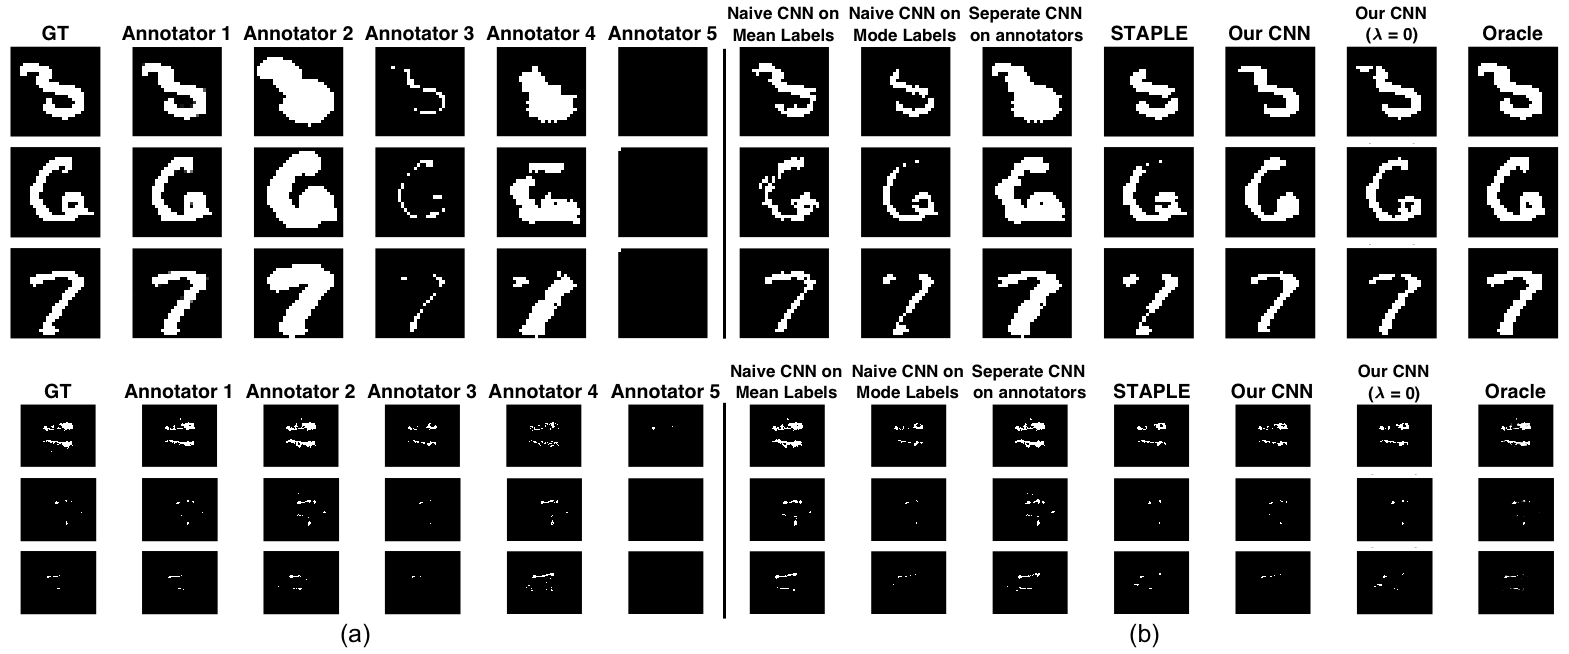
\includegraphics[width=\linewidth]{chapter_8_neurips/picture11.png}
    \vspace{-3mm}
    \caption{\footnotesize Visualisation of segmentation labels on two datasets: (a) ground-truth (GT) and segmentation labels from simulated annotators (Annotators 1 - 5); (b) the predictions from the supervised models.}
    \label{MNIST and MS segmentation results}
    \vspace{-2mm}
\end{figure}


\section{Experiments}

\paragraph{Datasets}
We evaluate our method on a variety of datasets including both synthetic and real-world scenarios: 1) for MNIST segmentation and ISBI2015 MS lesion segmentation challenge dataset \cite{jesson2015hierarchical}, we apply morphological operations to simulate different types of annotation noise in binary segmentation tasks; 2) for the BraTS 2019 brain tumour segmentation dataset \cite{menze2014multimodal}, we perform a similar simulation in a multi-class segmentation task; 3) we also consider the LIDC-IDRI dataset which contains real noisy annotations acquired from 4 different clinical experts. 

We simulate a group of 5 annotators of disparate characteristics by performing morphological transformations (e.g., thinning, thickening, fractures, etc) on the ground-truth (GT) segmentation labels, using Morpho-MNIST software \cite{castro2019morphomnist}. In particular, the first annotator provides faithful segmentation (``good-segmentation'') with approximate GT, the second tends over-segment (``over-segmentation''), the third tends to under-segment (``under-segmentation''), the fourth is prone to the combination of small fractures and over-segmentation (``wrong-segmentation'') and the fifth always annotates everything as the background (``blank-segmentation''). To create synthetic noisy labels in multi-class scenario, we first choose a target class and then apply morphological operations on the provided GT mask to create 4 synthetic noisy labels at different patterns, namely, over-segmentation, under-segmentation, wrong segmentation and good segmentation. We create training data by deriving labels from the simulated annotators. We also experimented with varying the levels of morphological operations on MNIST and MS lesion datasets, to test the robustness of our methods to varying degrees of annotation noise.


\paragraph{Baselines}
Our experiments are based on the assumption that no ground-truth (GT) label is not known a priori, hence, we compare our method against multiple label fusion methods. In particular, we consider four label fusion baselines: a) mean of all of the noisy labels; b) mode labels by taking the ``majority vote''; c) label fusion via the original STAPLE method \cite{warfield2004simultaneous}; d) Spatial STAPLE, a more recent extension of c) that accounts for spatial variations in CMs. After curating the noisy annotations via the above methods, we train the segmentation network and report the results. For c) and d), we used the toolkit\footnote{https://www.nitrc.org/projects/masi-fusion/}. To get an upper-bound performance, we also include the \textit{oracle} model that is directly trained on the ground-truth annotations. To test the value of the proposed image-dependent spatial CMs, we also include ``Global CM'' model where a single CM is learned per annotator but fixed across pixels and images (analogous to \etal \cite{raykar2009supervised,khetan2017learning,tanno2019learning}, but in segmentation task). Lastly, we also compare against a recent method called Probabilistic U-net as another baseline, which has been shown to capture inter-reader variations accurately. The details are presented in Appendix \ref{Appendix MNIST and MS}. 

\paragraph{Metrics}
For evaluation metrics, we use: 1) root-MSE between estimated CMs and real CMs; 2) Dice coefficient (DICE) between estimated segmentation and true segmentation; 3) The generalized energy distance proposed in \cite{kohl2018probabilistic} to measure the quality of the estimated annotator's labels.  



\paragraph{Implementation}
Our method as well as the above baselines are implemented in Pytorch. Our network is based on a 4 down-sampling stages 2D U-net \cite{ronneberger2015u}, the channel numbers for each encoders are 32, 64, 128, 256, we also replaced the batch normalisation layers with instance normalisation. Our segmentation network and annotator network share the same parameters apart from the last layer in the decoder of U-net, essentially, the overall architecture is implemented as an U-net with multiple output last layers: one for prediction of true segmentation; others for predictions of noisy segmentation respectively. For segmentation network, the output of the last layer has c channels where c is the number of classes. On the other hand, for annotator network, by default, the output of the last layer has  $L \times L$ number of channels for estimating confusion matrices at each spatial location; when low-rank approximation is used, the output of the last layer has 2 $\times$ L $\times l$  number of channels. The Probabilistic U-net implementation is adopted from \url{https://github.com/stefanknegt/Probabilistic-Unet-Pytorch}, for fair comparison, we adjusted the number of the channels and the depth of the U-net backbone in Probabilistic U-net to match with our networks. All of the models were trained on a NVIDIA RTX 208 for at least 3 times with different random initialisations to compute the mean performance and its standard deviation (run 3 times of the experiments with the same initialization). The Adam \cite{kingma2014adam} optimiser was used in all experiments with the default hyper-parameter settings. We also provide all of the hyper-parameters of the experiments for each data set in Table~\ref{Experiments_settings}. We also kept the training details the same between the baselines and our method.
\vspace{-2mm}
\begin{table}[!h]
	\center
	\footnotesize
	\begin{tabular}{@{}lllllc}
		\hline
		 Data set & Learning Rate & Epoch & Batch Size & Augmentation & weight for regularisation ($\lambda$) \\
		\hline	
		MNIST  & 1e-4  & 60 & 2 & Random flip & 0.7 \\
		MS & 1e-4 & 55  & 2 & Random flip & 0.7\\
		BraTS & 1e-4 & 60 & 8 & Random flip & 1.5 \\
		LIDC & 1e-4  & 75 & 4 & Random flip & 0.9 \\
		\hline
	\end{tabular}%
\caption{\footnotesize Hyper-parameters used for respective datasets.}
\label{Experiments_settings}
\end{table}


\subsection{MNIST and MS lesion segmentation datasets}
MNIST dataset consists of 60,000 training and 10,000 testing examples, all of which are 28 $\times$ 28 grayscale images of digits from 0 to 9, and we derive the segmentation labels by thresholding the intensity values at 0.5. The MS dataset is publicly available and comprises 21 3D scans from 5 subjects. All scans are split into 10 for training and 11 for testing. We hold out 20\% of training images as a validation set for both datasets. On both datasets, our proposed model achieves a higher dice similarity coefficient than STAPLE on the dense label case and, even more prominently, on the single label (i.e., randomly choose 1 label per image, aka, ``one label per image'') case (shown in Tables.~\ref{denselabel of MNIST and MS}\&\ref{singlelabel of MNIST and MS} and Fig.~\ref{MNIST and MS segmentation results}). In addition, our model outperforms STAPLE without or with trace norm, in terms of CM estimation, specifically, we could achieve an increase at $6.3\%$. Additionally, we include the performance on different regularisation coefficient, which is presented in Fig.~\ref{Paramater lambda}. Fig.~\ref{plot of denselabel and single label} compares the segmentation accuracy on MNIST and MS lesion for a range of average dice where labels are generated by a group of 5 simulated annotators. Fig.~\ref{CMs of MNIST and MS} illustrates our model can capture the patterns of mistakes for each annotator. We also notice that our model is consistently more accurate than the global CM model, indicating the value of image-dependent pixel-wise CMs. 


\begin{table}[!h]
\vspace{-4mm}
	\center
	\footnotesize
	\begin{tabular}{@{}lllllllll}
		\hline
		 & MNIST & MNIST  & MSLesion  & MSLesion  \\
		Models & DICE (\%) & CM estimation & DICE (\%) & CM estimation \\
		\hline	
		Naive CNN on mean labels & 38.36 $\pm$ 0.41 &  n/a & 46.55 $\pm$ 0.53 &  n/a  \\
		Naive CNN on mode labels & 62.89 $\pm$ 0.63 &  n/a & 47.82 $\pm$ 0.76 &  n/a  \\
		Probabilistic U-net \cite{kohl2018probabilistic}  & 65.12 $\pm$ 0.83  &  n/a  & 46.15 $\pm$ 0.59  & n/a    \\
		Separate CNNs on annotators & 70.44 $\pm$ 0.65 & n/a & 46.84 $\pm$ 1.24 & n/a &   \\ 
		STAPLE \cite{warfield2004simultaneous}& 78.03 $\pm$ 0.29 &  0.1241 $\pm$ 0.0011 & 55.05 $\pm$ 0.53 &  0.1502 $\pm$ 0.0026 \\ 
		Spatial STAPLE \cite{asman2012formulating} & 78.96 $\pm$ 0.22 &  0.1195 $\pm$ 0.0013 & 58.37 $\pm$ 0.47 &  0.1483 $\pm$ 0.0031  \\
		Ours with Global CMs & 79.21 $\pm$ 0.41  & 0.1132 $\pm$ 0.0028 & 61.58 $\pm$ 0.59   &  0.1449 $\pm$ 0.0051   \\
		Ours without Trace & 79.63 $\pm$ 0.53  &  0.1125 $\pm$ 0.0037 & 65.77 $\pm$ 0.62 &  0.1342 $\pm$ 0.0053  \\
		Ours & 82.92 $\pm$ 0.19 &  0.0893 $\pm$ 0.0009 & 67.55 $\pm$ 0.31 &  0.0811 $\pm$ 0.0024    \\
		Oracle (Ours but with known CMs)   & 83.29 $\pm$ 0.11 & 0.0238 $\pm$ 0.0005 & 78.86 $\pm$ 0.14 &  0.0415 $\pm$ 0.0017   \\ 
		\hline
	\end{tabular}%
\caption{\footnotesize Comparison of segmentation accuracy (DICE) and quality of confusion matrix (CM) estimation (MSE) for different methods with dense labels (mean $\pm$ standard deviation).}
\label{denselabel of MNIST and MS}
\end{table}
\vspace{-4mm}
\begin{table}[t!]
	\center
	\footnotesize
	\begin{tabular}{@{}llllllllll}
		\hline
		 & MNIST & MNIST  & MSLesion  & MSLesion  \\
		Models & DICE (\%) & CM estimation & DICE (\%) & CM estimation \\
		  
		\hline	
		Naive CNN & 32.79 $\pm$ 1.13 &  n/a & 27.41 $\pm$ 1.45 &  n/a  \\
		STAPLE \cite{warfield2004simultaneous}& 54.07 $\pm$ 0.68 &  0.2617 $\pm$ 0.0064& 35.74 $\pm$ 0.84 &  0.2833 $\pm$ 0.0081  \\ 
		Spatial STAPLE \cite{asman2012formulating} & 56.73 $\pm$ 0.53 &  0.2384 $\pm$ 0.0061& 38.21 $\pm$ 0.71 &  0.2591 $\pm$ 0.0074  \\
 		Ours with Global CMs  & 59.01 $\pm$ 0.65   & 0.1953 $\pm$ 0.0041   & 40.32 $\pm$ 0.68  & 0.1974 $\pm$ 0.0063    \\
		Ours without Trace & 74.48 $\pm$ 0.37  &  0.1538 $\pm$ 0.0029 & 54.76 $\pm$ 0.66 & 0.1745 $\pm$ 0.0044  \\
		Ours & 76.48 $\pm$ 0.25  &  0.1329 $\pm$ 0.0012 & 56.43 $\pm$ 0.47 &  0.1542 $\pm$ 0.0023  \\
		\hline
	\end{tabular}%
\caption{\small Comparison of segmentation accuracy (DICE) and error of CM estimation (MSE) for different methods with one label per image (mean $\pm$ standard deviation).  We note that `Naive CNN' is a baseline trained by simply minimising the cross-entropy between the predictions and the noisy labels. }
\label{singlelabel of MNIST and MS}
\vspace{-4mm}
\end{table}
\vspace{-4mm}

\begin{figure}[t!]
        \center
        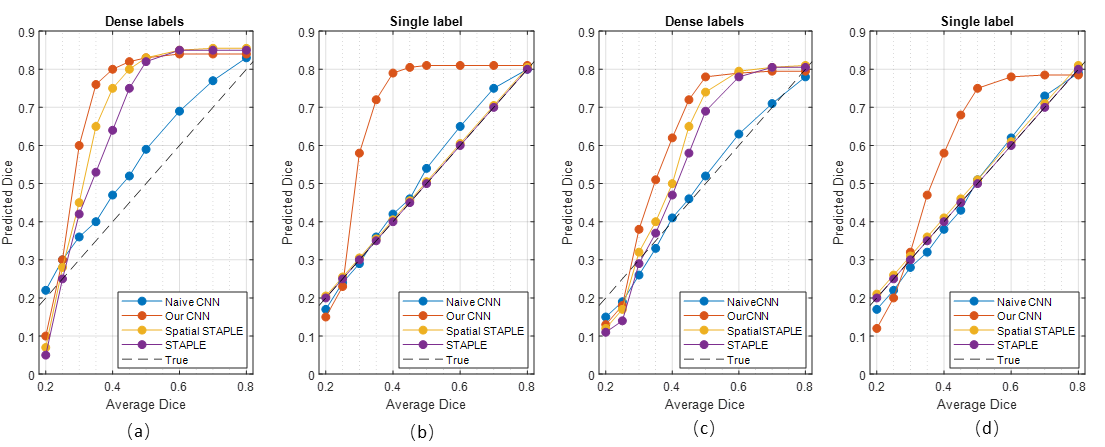
\includegraphics[width=\linewidth]{chapter_8_neurips/picture3.png}
        \caption{Segmentation accuracy of different models on MNIST (a, b) and MS (c, d) dataset for a range of annotation noise (measured in averaged Dice with respect to GT.}
        \label{plot of denselabel and single label}
\end{figure}

\begin{figure}[t!]
        \center
        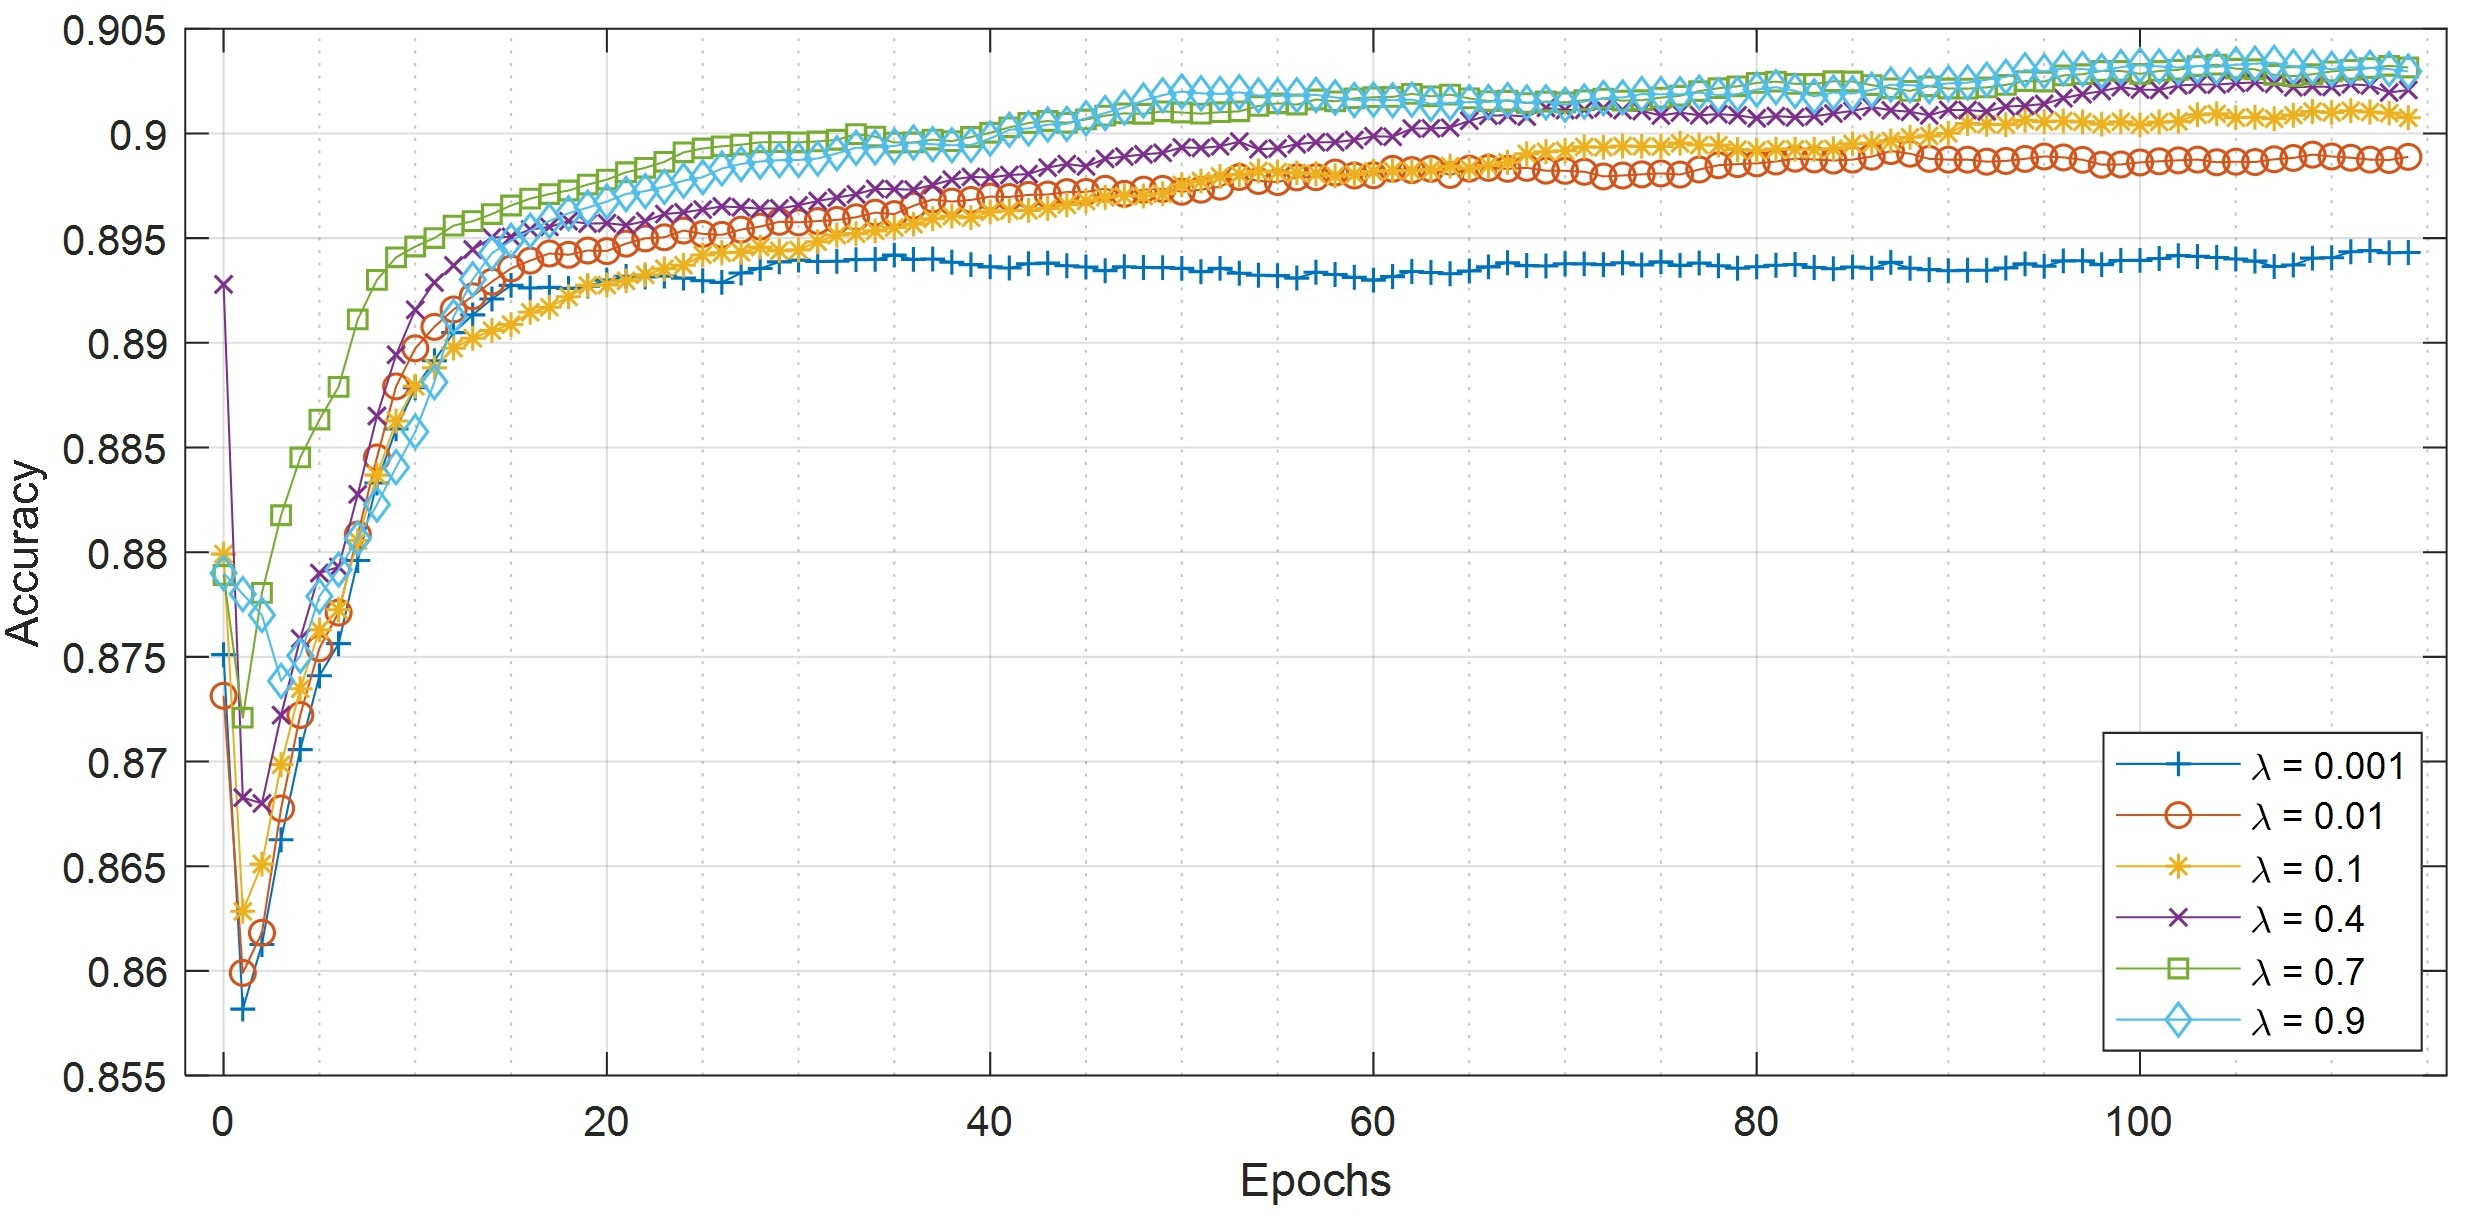
\includegraphics[width=\linewidth]{chapter_8_neurips/picture4.jpg}
        \caption{Curves of validation accuracy during training of our model on MNIST for a range of hyperparameters. For our method, the scaling of trace regularizer is varied in [0.001, 0.01, 0.1, 0.4, 0.7, 0.9].)}
        \label{Paramater lambda}
\end{figure}
    

\begin{figure}[t!]
    \centering
    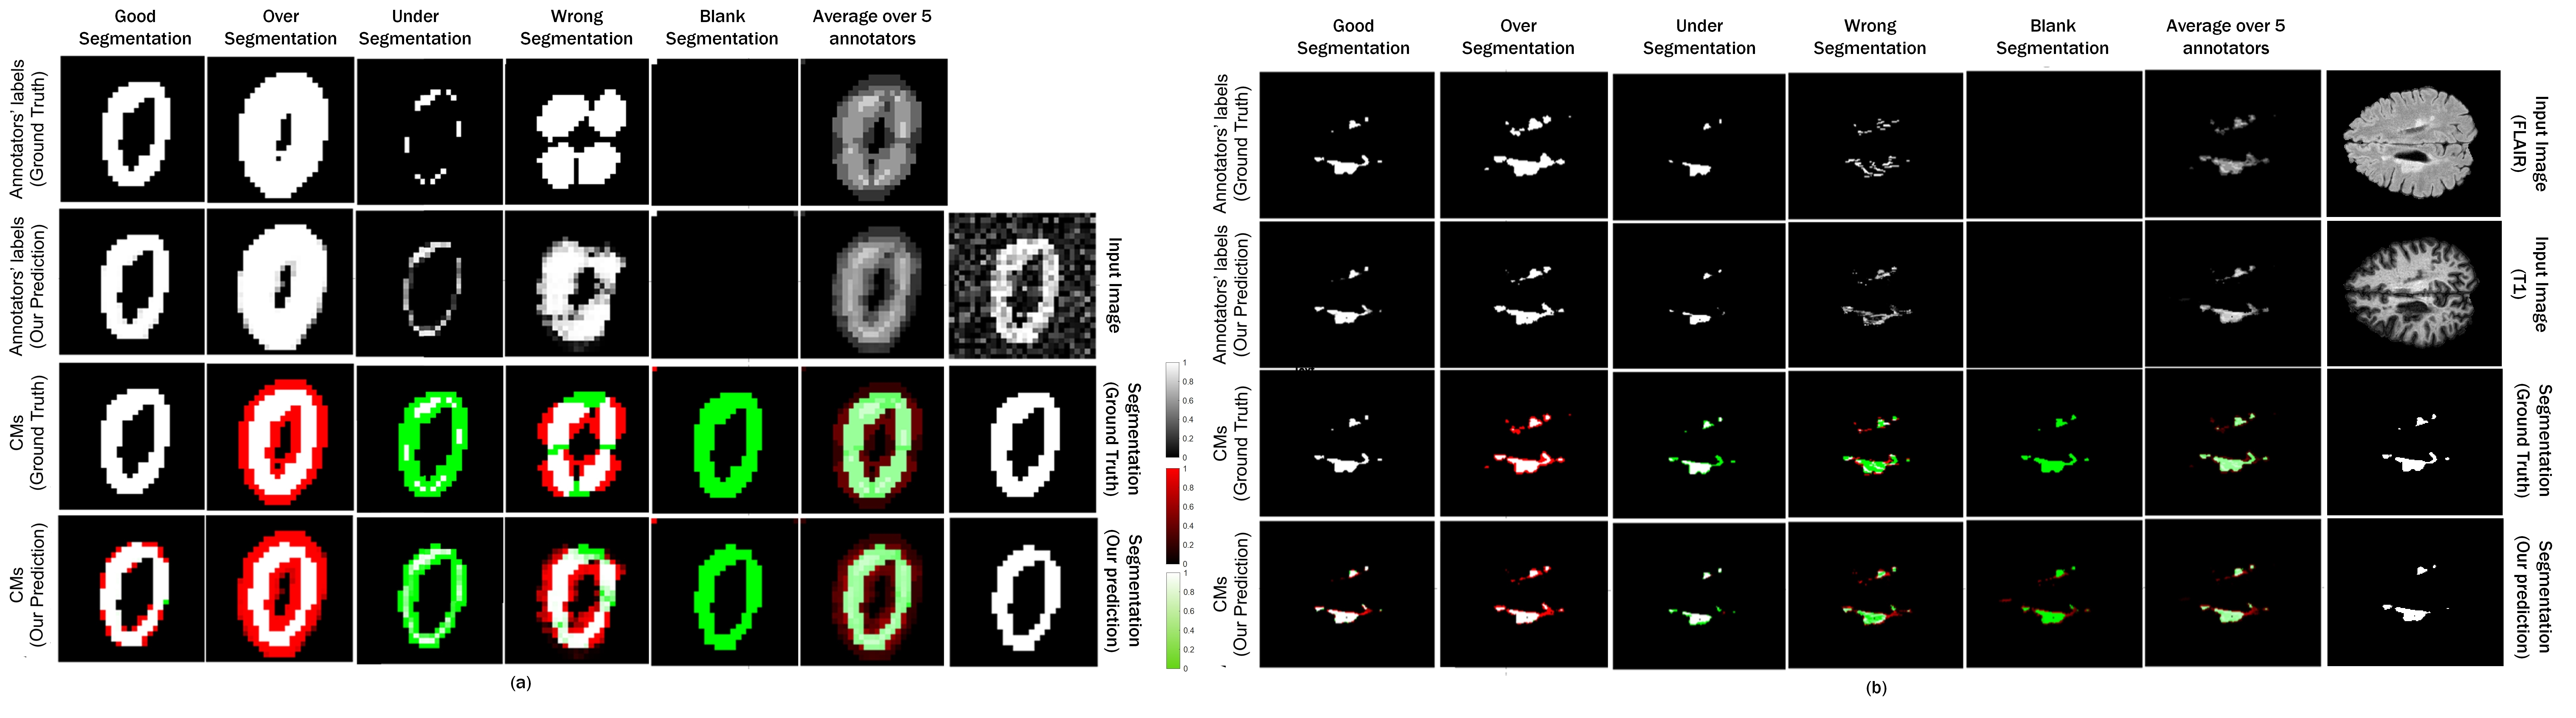
\includegraphics[width=\linewidth]{chapter_8_neurips/picture7.jpg}
    \caption{\footnotesize Visualisation of the estimated true labels and the estimated pixel-wise confusion matrices on MNIST/MS datasets along with their targets (best viewed in colour). White is the true positive, green is the false negative, red is the false positive and black is the true negative.}
    \label{CMs of MNIST and MS}
\end{figure}

\clearpage
\subsection{BraTS Dataset and LIDC-IDRI Dataset}
We also evaluate our model on a multi-class segmentation task, using all of the 259 high grade glioma (HGG) cases in training data from 2019 multi-modal Brain Tumour Segmentation Challenge (BraTS). We extract each slice as 2D images and split them at case-wise to have, 1600 images for training, 300 for validation and 500 for testing. Pre-processing includes: concatenation of all of available modalities; centre cropping to 192 x 192; normalisation for each case at each modality. To create synthetic noisy labels in multi-class scenario, we first choose a target class and then apply morphological operations on the provided GT mask to create 4 synthetic annotators of different characteristics. Some examples are shown in Fig.~\ref{Brats results segmentation2}(a). 

\begin{table}[H]
	\center
	\scriptsize
	\begin{tabular}{@{}lllllllll}
		\hline
		 & BraTS & BraTS  & LIDC-IDRI  & LIDC-IDRI  \\
		Models & DICE (\%) & CM estimation & DICE (\%) & CM estimation \\
		  
		\hline	
		Naive CNN on mean labels & 29.42 $\pm$ 0.58  &  n/a & 56.72 $\pm$ 0.61  &  n/a  \\
		Naive CNN on mode labels & 34.12 $\pm$ 0.45  &  n/a & 58.64 $\pm$ 0.47  &  n/a  \\
		Probabilistic U-net \cite{kohl2018probabilistic}  & 40.53 $\pm$ 0.75   &  n/a  & 61.26 $\pm$ 0.69  &  n/a   \\
		STAPLE \cite{warfield2004simultaneous}& 46.73 $\pm$ 0.17  & 0.2147 $\pm$ 0.0103   & 69.34 $\pm$ 0.58  & 0.0832 $\pm$ 0.0043   \\ 
		Spatial STAPLE \cite{asman2012formulating} & 47.31 $\pm$ 0.21  & 0.1871 $\pm$ 0.0094   & 70.92 $\pm$ 0.18  &  0.0746 $\pm$ 0.0057   \\
		Ours with Global CMs &  47.33 $\pm $ 0.28  &  0.1673 $\pm $ 0.1021    & 70.94 $\pm $ 0.19  & 0.1386 $\pm $ 0.0052   \\
		Ours without Trace & 49.03 $\pm$ 0.34   & 0.1569 $\pm$ 0.0072   & 71.25 $\pm$ 0.12  & 0.0482 $\pm$ 0.0038    \\
		Ours & \textbf{53.47 $\pm $ 0.24}  & \textbf{0.1185 $\pm$ 0.0056 }  & \textbf{74.12 $\pm $ 0.19 } &  \textbf{0.0451 $\pm$ 0.0025     }\\
		Oracle (Ours but with known CMs)   & 67.13 $\pm$ 0.14  & 0.0843 $\pm$ 0.0029  & 79.41 $\pm$ 0.17  & 0.0381 $\pm$ 0.0021    \\ 
		\hline
	\end{tabular}%
	\vspace{1mm}
    \caption{\footnotesize Comparison of segmentation accuracy and error of CM estimation for different methods trained with \textbf{dense labels} (mean $\pm$ standard deviation). The best results are shown in bald. Note that we count out the Oracle from the model ranking as it forms a theoretical upper-bound on the performance where true labels are known on the training data.}
\label{denselabebrats}
\end{table}
\vspace{-5mm}
\begin{table}[H]
	\center
	\scriptsize
	\begin{tabular}{@{}llllllllll}
		\hline
		 & BraTS & BraTS  & LIDC-IDRI  & LIDC-IDRI  \\
		Models & DICE (\%) & CM estimation & DICE (\%) & CM estimation \\
		  
		\hline	
		Naive CNN on mean \& mode labels& 36.12 $\pm$ 0.93  &  n/a & 48.36 $\pm$ 0.79   &  n/a  \\
		STAPLE \cite{warfield2004simultaneous}& 38.74 $\pm$ 0.85  & 0.2956 $\pm$ 0.1047  & 57.32 $\pm$ 0.87  & 0.1715 $\pm$ 0.0134     \\ 
		Spatial STAPLE \cite{asman2012formulating} & 41.59 $\pm$ 0.74  & 0.2543 $\pm$ 0.0867  & 62.35 $\pm$ 0.64  & 0.1419 $\pm$ 0.0207    \\
 		Ours with Global CMs  & 41.76 $\pm$ 0.71  & 0.2419 $\pm$ 0.0829   & 63.25 $\pm$ 0.66  & 0.1382 $\pm$ 0.0175    \\
		Ours without Trace & 43.74 $\pm$ 0.49   & 0.1825 $\pm$ 0.0724   & 66.95 $\pm$ 0.51  & 0.0921 $\pm$ 0.0167   \\
		Ours & \textbf{46.21 $\pm$ 0.28}   & \textbf{0.1576 $\pm$ 0.0487 }  & \textbf{68.12 $\pm$ 0.48}  & \textbf{0.0587 $\pm$ 0.0098   } \\
		\hline
	\end{tabular}%
		\vspace{1mm}
    \caption{\footnotesize Comparison of segmentation accuracy and error of CM estimation for different methods trained with only one label available per image (mean $\pm$ standard deviation). The best results are shown in bald.}
    \label{singlelabebrats}
\end{table}

\begin{figure}[t!]
    \centering
    \includegraphics[width=\linewidth]{chapter_8_neurips/picture16.jpg}
    \caption{Visualisation of segmentation labels on BraTS dataset: (a) GT and simulated annotator's segmentations (Annotator 1 - 5); (b) the predictions from the supervised models.) }
    \label{Brats results segmentation2}
\end{figure}


\begin{figure}[t!]
    \centering
    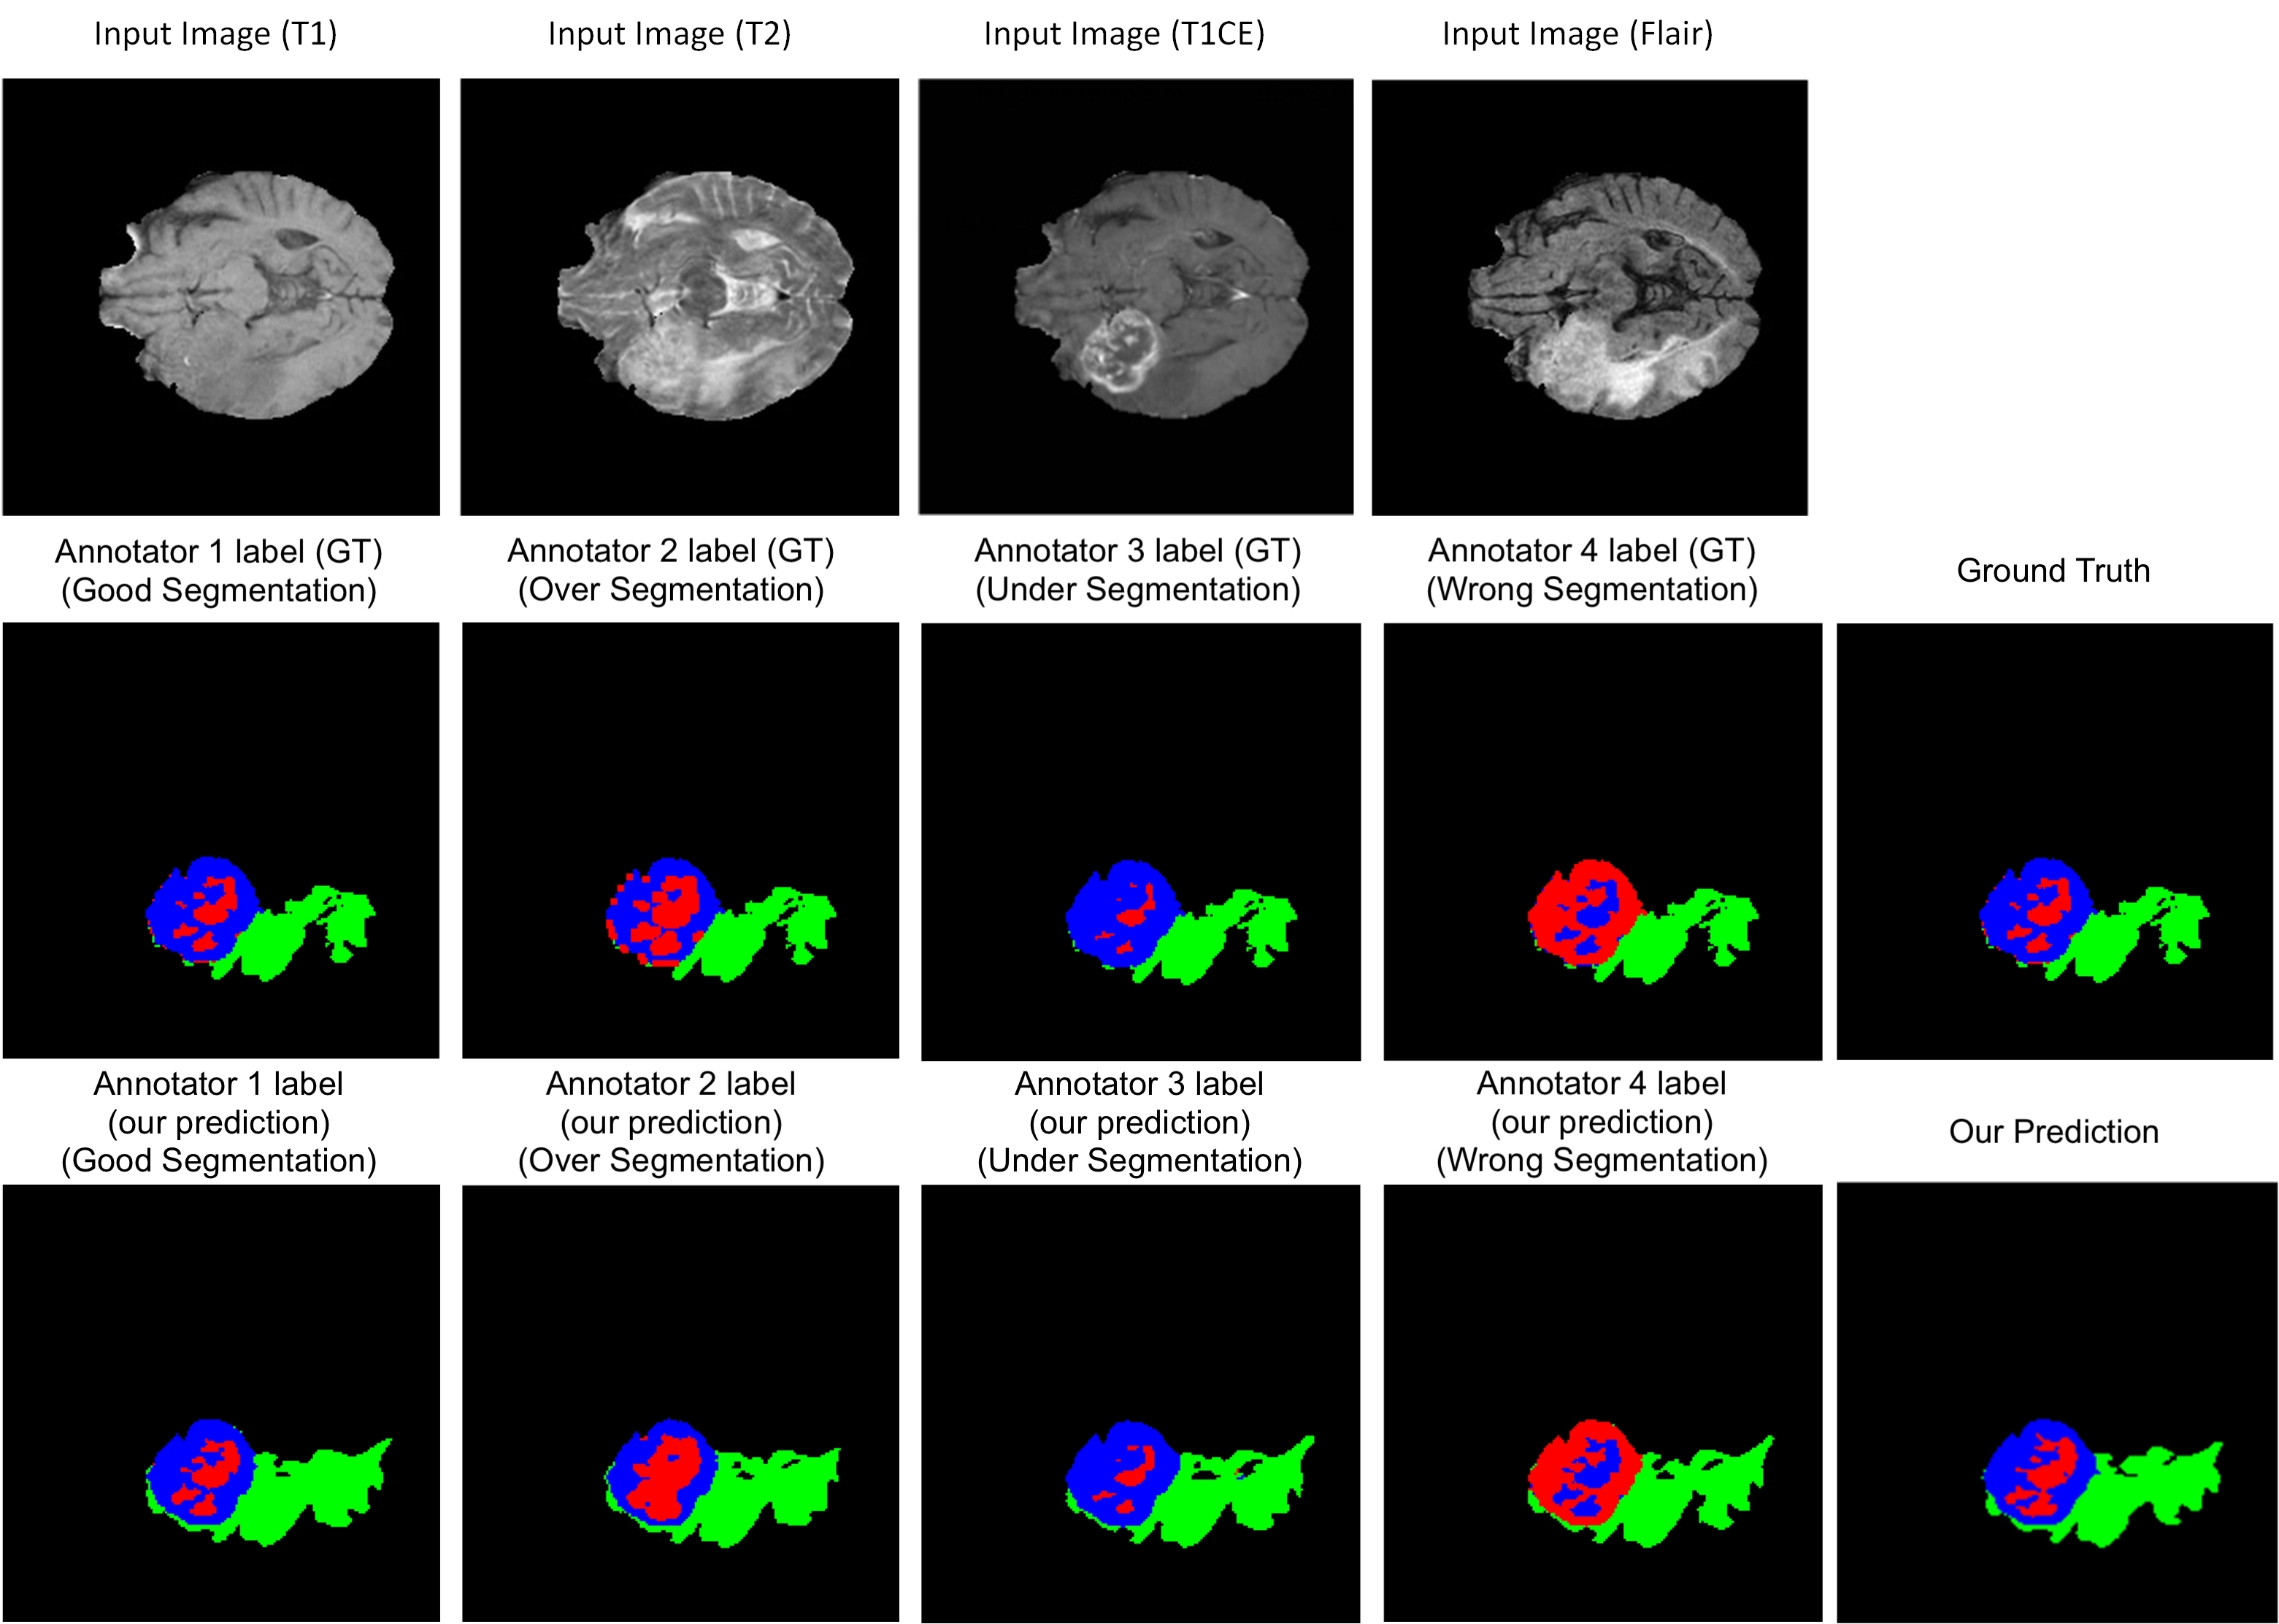
\includegraphics[width=\linewidth]{chapter_8_neurips/picture8.jpg}
        \caption{\footnotesize Visualisation of the estimated true segmentation on the BraTS dataset and the estimated annotations of their respective annotators (best viewed in colour). The tumour core (red) is the target class on which annotation mistakes are simulated.}
        \label{Brats results}
\end{figure}


Lastly, we use the LIDC-IDRI dataset to evaluate the method in the scenario where multiple labels are actually acquired from different clinical experts. The dataset contains 1018 lung CT scans from 1010 lung patients with manual lesion segmentations from four experts. %This dataset is a good representation of the typical ambiguities that appear in CT scans. 
For each scan, 4 radiologists provided annotation masks for lesions that they independently detected and considered to be abnormal. For our experiments, we used the same method in \cite{kohl2018probabilistic} to pre-process all scans. We split the dataset at case-wise into a training (722 patients), validation (144 patients) and testing (144 patients). We then resampled the CT scans to $1 mm \times 1 mm$ in-plane resolution. We also centre cropped 2D images ($180 \times 180$ pixels) around lesion positions, in order to focus on the annotated lesions. The lesion positions are those where at least one of the experts segmented a lesion. We hold 5000 images in the training set, 1000 images in the validation set and 1000 images in the test set. Since the dataset does not provide a single curated ground-truth for each image, we created a ``gold standard'' by aggregating the labels via STAPLE \cite{asman2012formulating}, a recent variant of the STAPLE framework employed in the creation of public medical image segmentation datasets e.g., ISLES \cite{winzeck2018isles}, MSSeg \cite{commowick2018objective}, Gleason'19 \cite{gleason2019} datasets. We further note that, as before, we assume labels are only available to the model during training, but not at test time, thus label aggregation methods cannot be applied on the test examples. 


\begin{figure}[t!]
    \vspace{-3mm}
    \centering
    
\includegraphics[width=\linewidth]{chapter_8_neurips/picture17.jpg}
    \caption{\footnotesize Visualisation of segmentation labels on LIDC-IDRI dataset: (a) GT and simulated annotator's segmentations (Annotator 1 - 5); (b) the predictions from the supervised models.)} 
    \label{LIDC segmentation}
\end{figure}


\begin{figure}[t!]
        \centering
        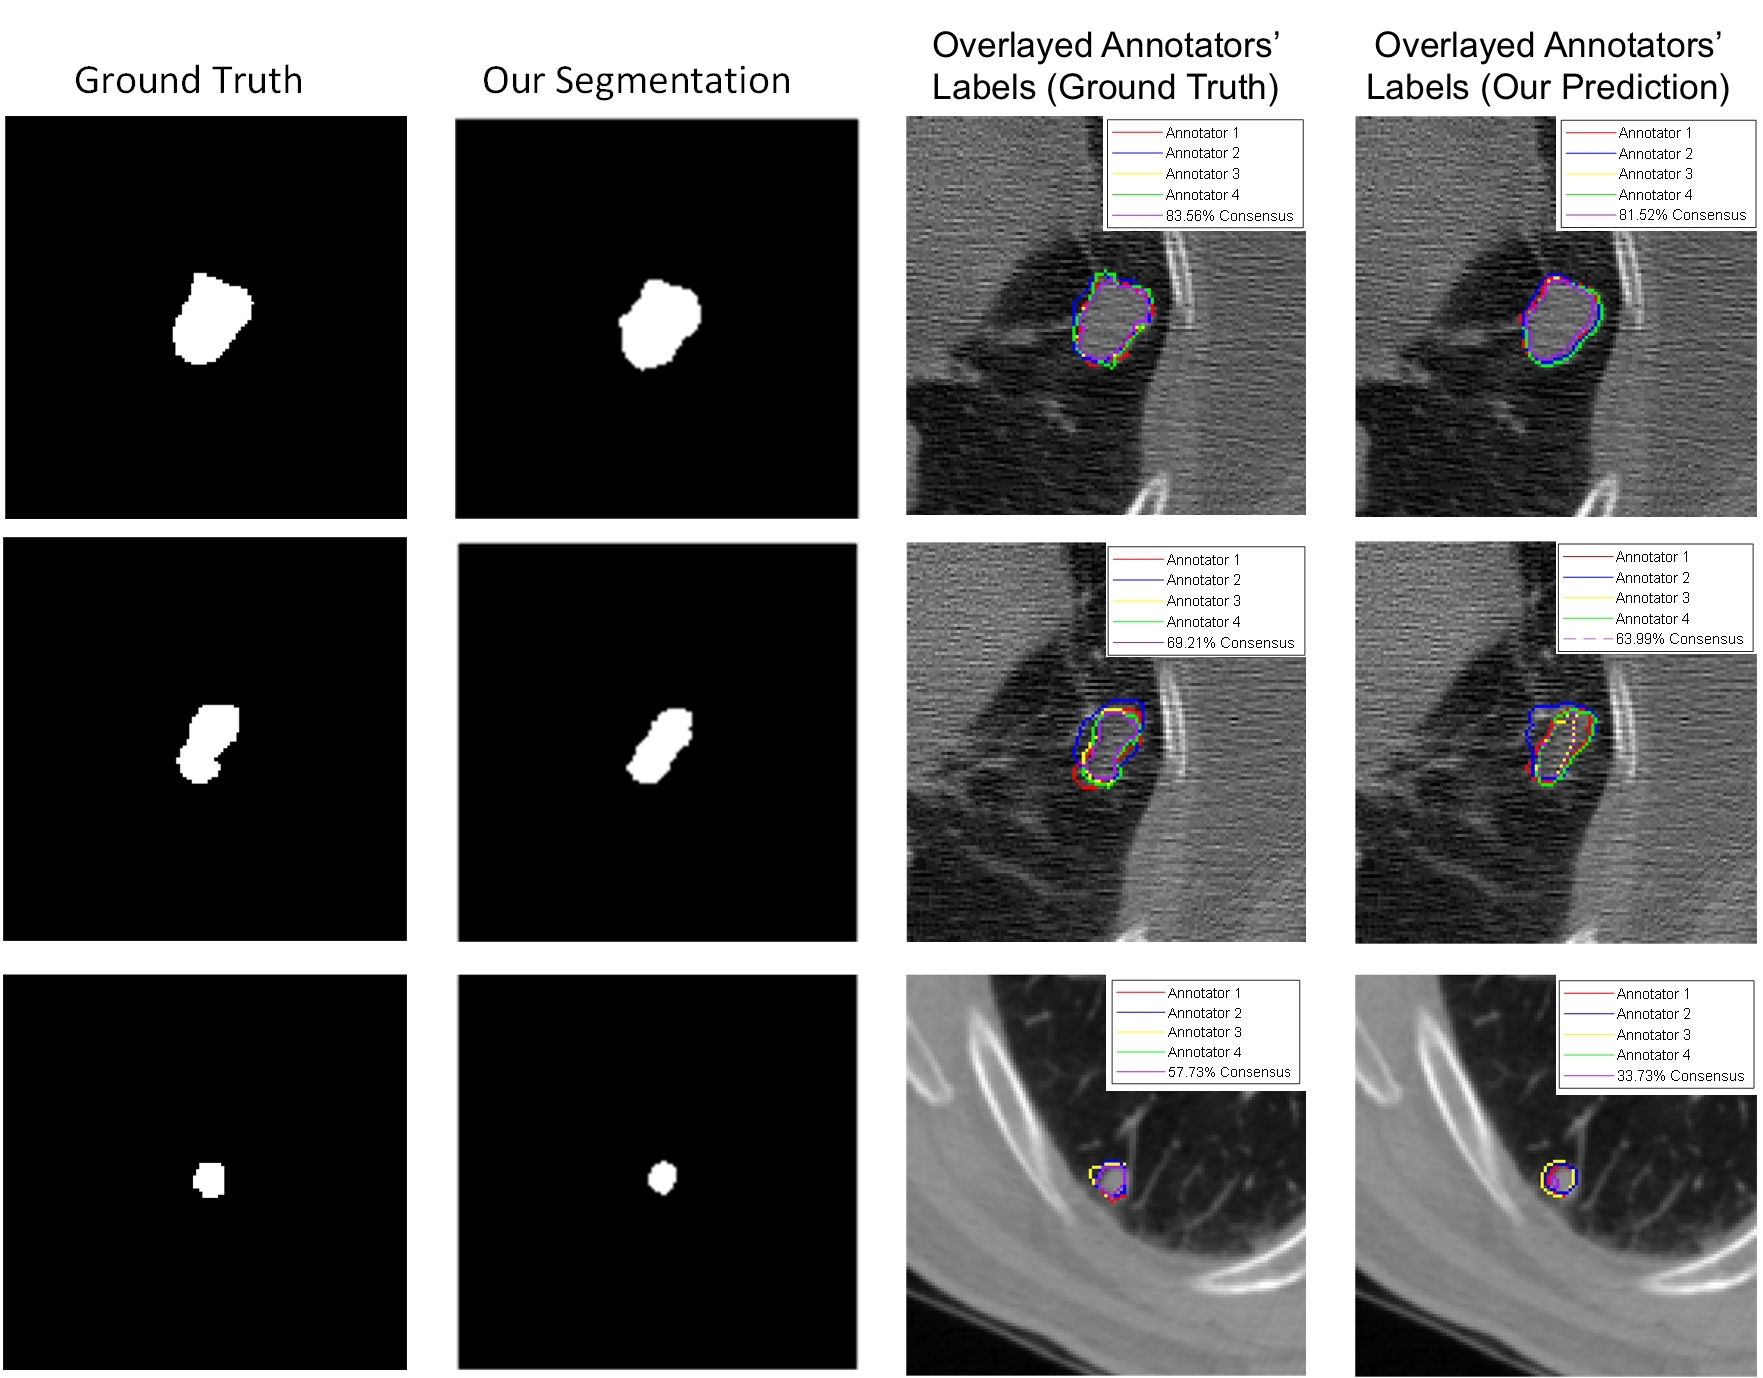
\includegraphics[width=0.9\linewidth]{chapter_8_neurips/picture10.jpg}
        \caption{\footnotesize Segmentation results on LIDC-IDRI dataset and the visualization of each annotator contours and the consensus. The bottom row shows an interesting example in which annotator 4 (green) misses the abnormality completely, which is also predicted by our model.}
        \label{LIDCresults}
\end{figure}


On both BraTS and LIDC-IDRI datasets, our proposed model achieves a higher dice similarity coefficient than STAPLE and Spatial STAPLE on both of the dense labels and single label scenarios (shown in Table. \ref{denselabebrats} and Table. \ref{singlelabebrats}). In addition, our model (with trace) outperforms STAPLE in terms of CM estimation by a large margin at $14.4\%$ on BraTS. In Fig. \ref{Brats results}, we visualize the segmentation results on BraTS and the corresponding annotators' predictions. Fig.~\ref{LIDCresults} presents three examples of the segmentation results and the corresponding four annotator contours, as well as the consensus. As shown in both figures, our model successfully predicts both the segmentation of lesions and the variations of each annotator in different cases. We also measure the inter-reader consensus levels by computing the IoU of multiple annotations, and compare the segmentation performance in 3 subgroups of different consensus levels (low, medium and high). Fig.~\ref{consensus dice} illustrates that 
our method attains consistent improvement over the baselines in all cases, indicating its ability to segment more robustly even the hard examples where the experts in reality have disagreed to a large extent. 

\begin{figure}[t!] 
	\center
        \begin{subfigure}[]{0.75\linewidth}
        		\caption{}
        		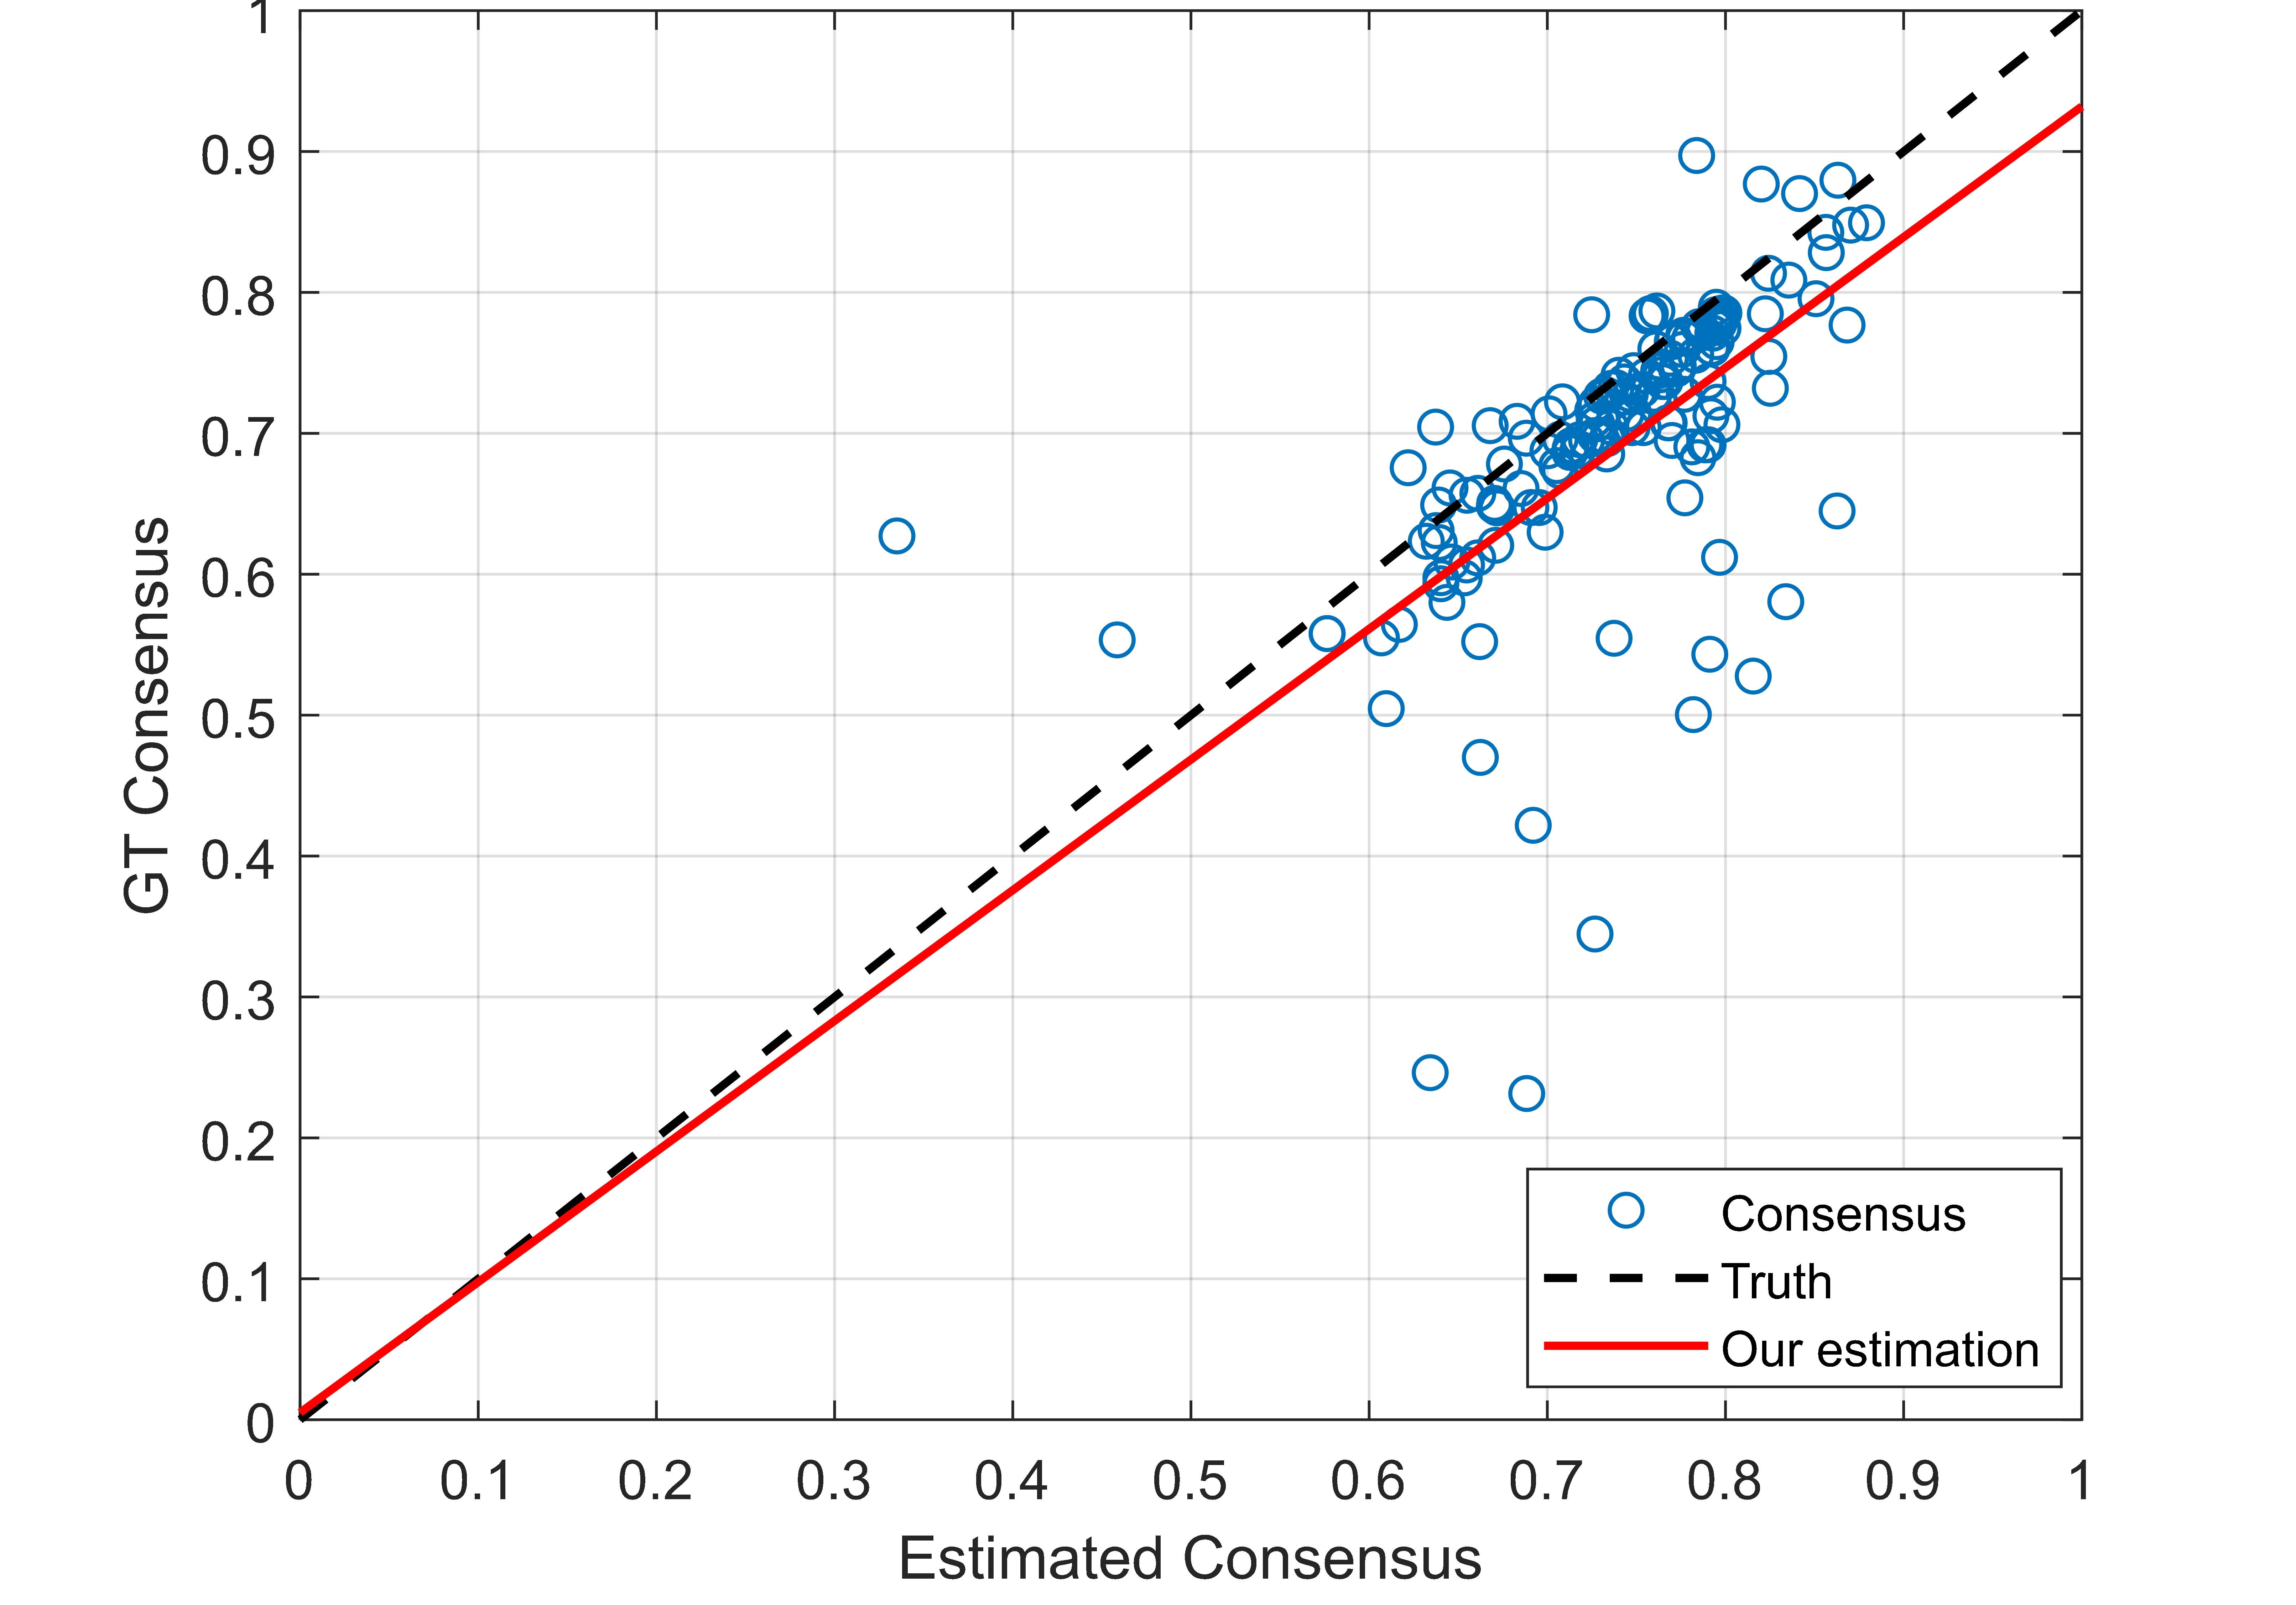
\includegraphics[width=\linewidth]{chapter_8_neurips/picture18.jpg}
        \end{subfigure}
        \hfill
        \begin{subfigure}[]{0.75\linewidth}         
	        \vspace{3mm}
	         \caption{}
	         \vspace{-3mm}
        		 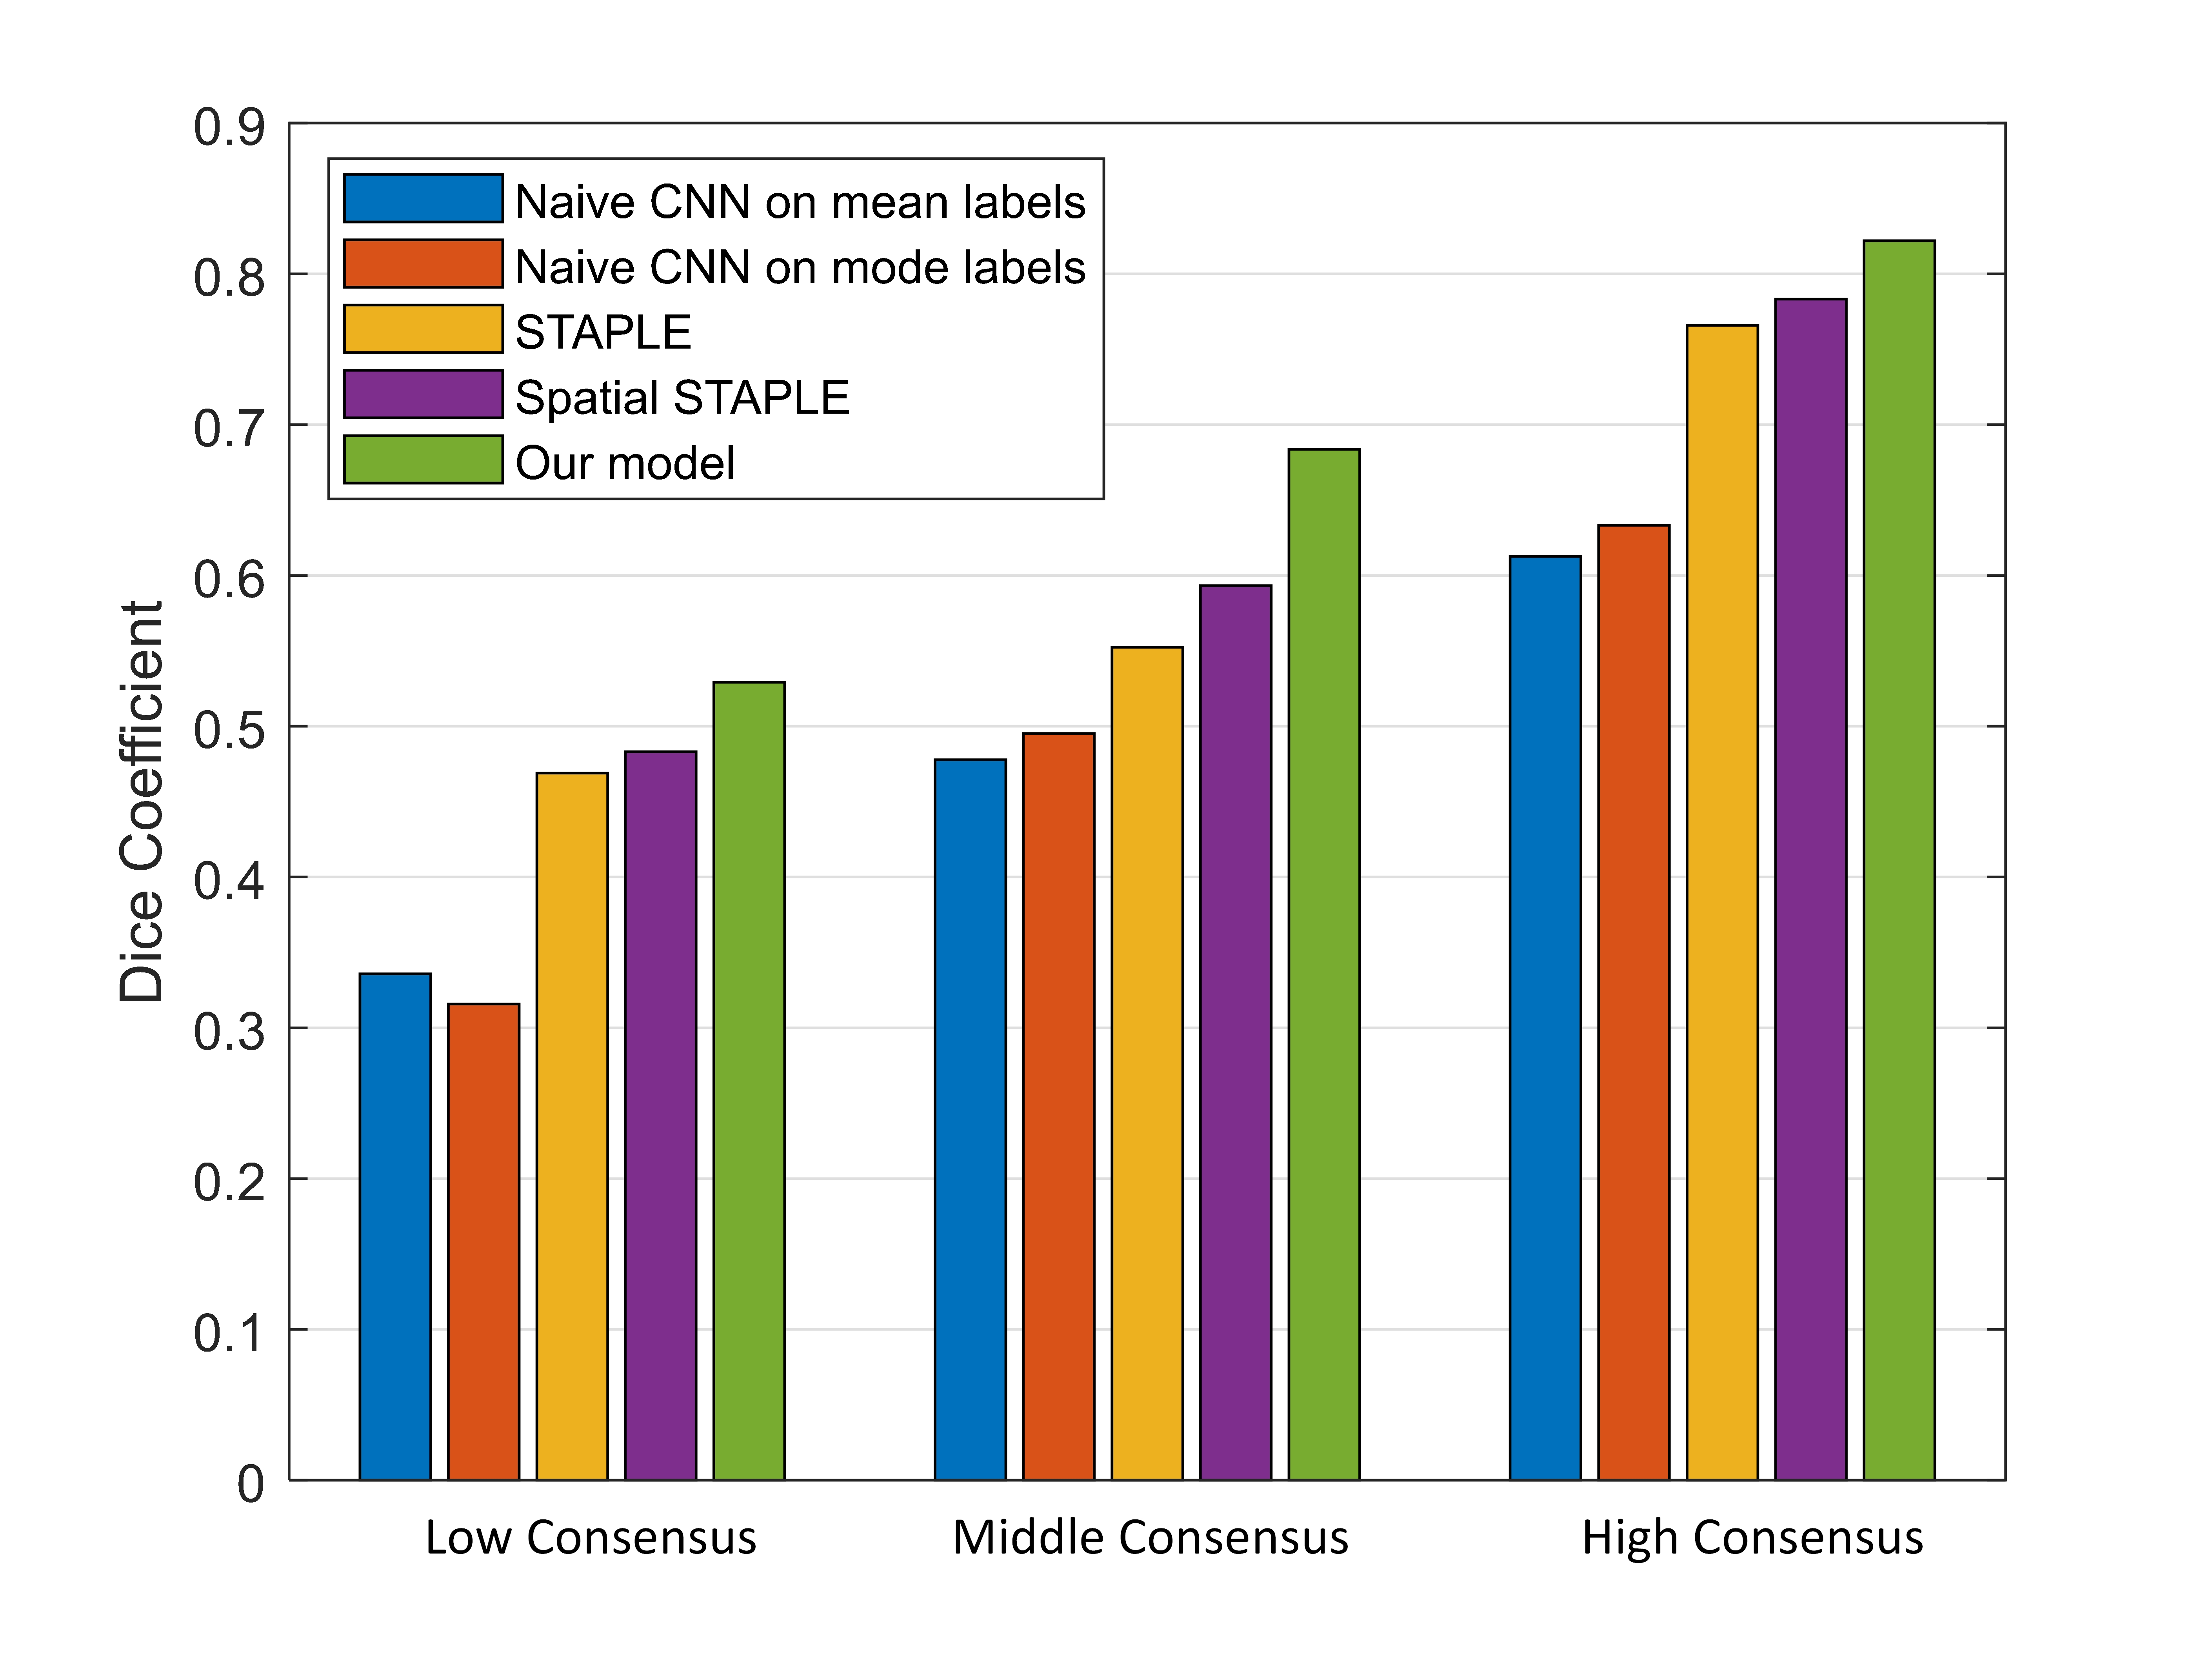
\includegraphics[width=\linewidth]{chapter_8_neurips/picture19.jpg}
        \end{subfigure}
       
        \caption{\footnotesize (a) The consensus level amongst the estimated annotators is plotted against the ground truth on LIDC-IDRI dataset. Here the inter-reader consensus level is measured as the IoU of available annotations. The strong positive linear correlation shows that the variation in the inter-reader variability on different input examples (e.g., some examples are more ambiguous than others) is captured well. We do note, however, that the inter-reader variation seems more under-estimated for ``easy'' (i.e., higher consensus) samples. (b) Segmentation performance on 3 different subgroups of the LIDC-IDRI dataset with varying levels of inter-reader agreement: 1) Low-consensus (30\% to 65\% IoU); 2) Middle consensus (65\% to 75\% IoU); 3) High consensus (75\% to 90\% IoU). Our method shows \textit{consistent} improvement over the baselines and the competing methods in all groups, showing its enhanced ability to segment challenging examples (i.e., low-consensus cases). }
        \label{consensus dice}
\end{figure}

%\begin{figure}
%        \center
%        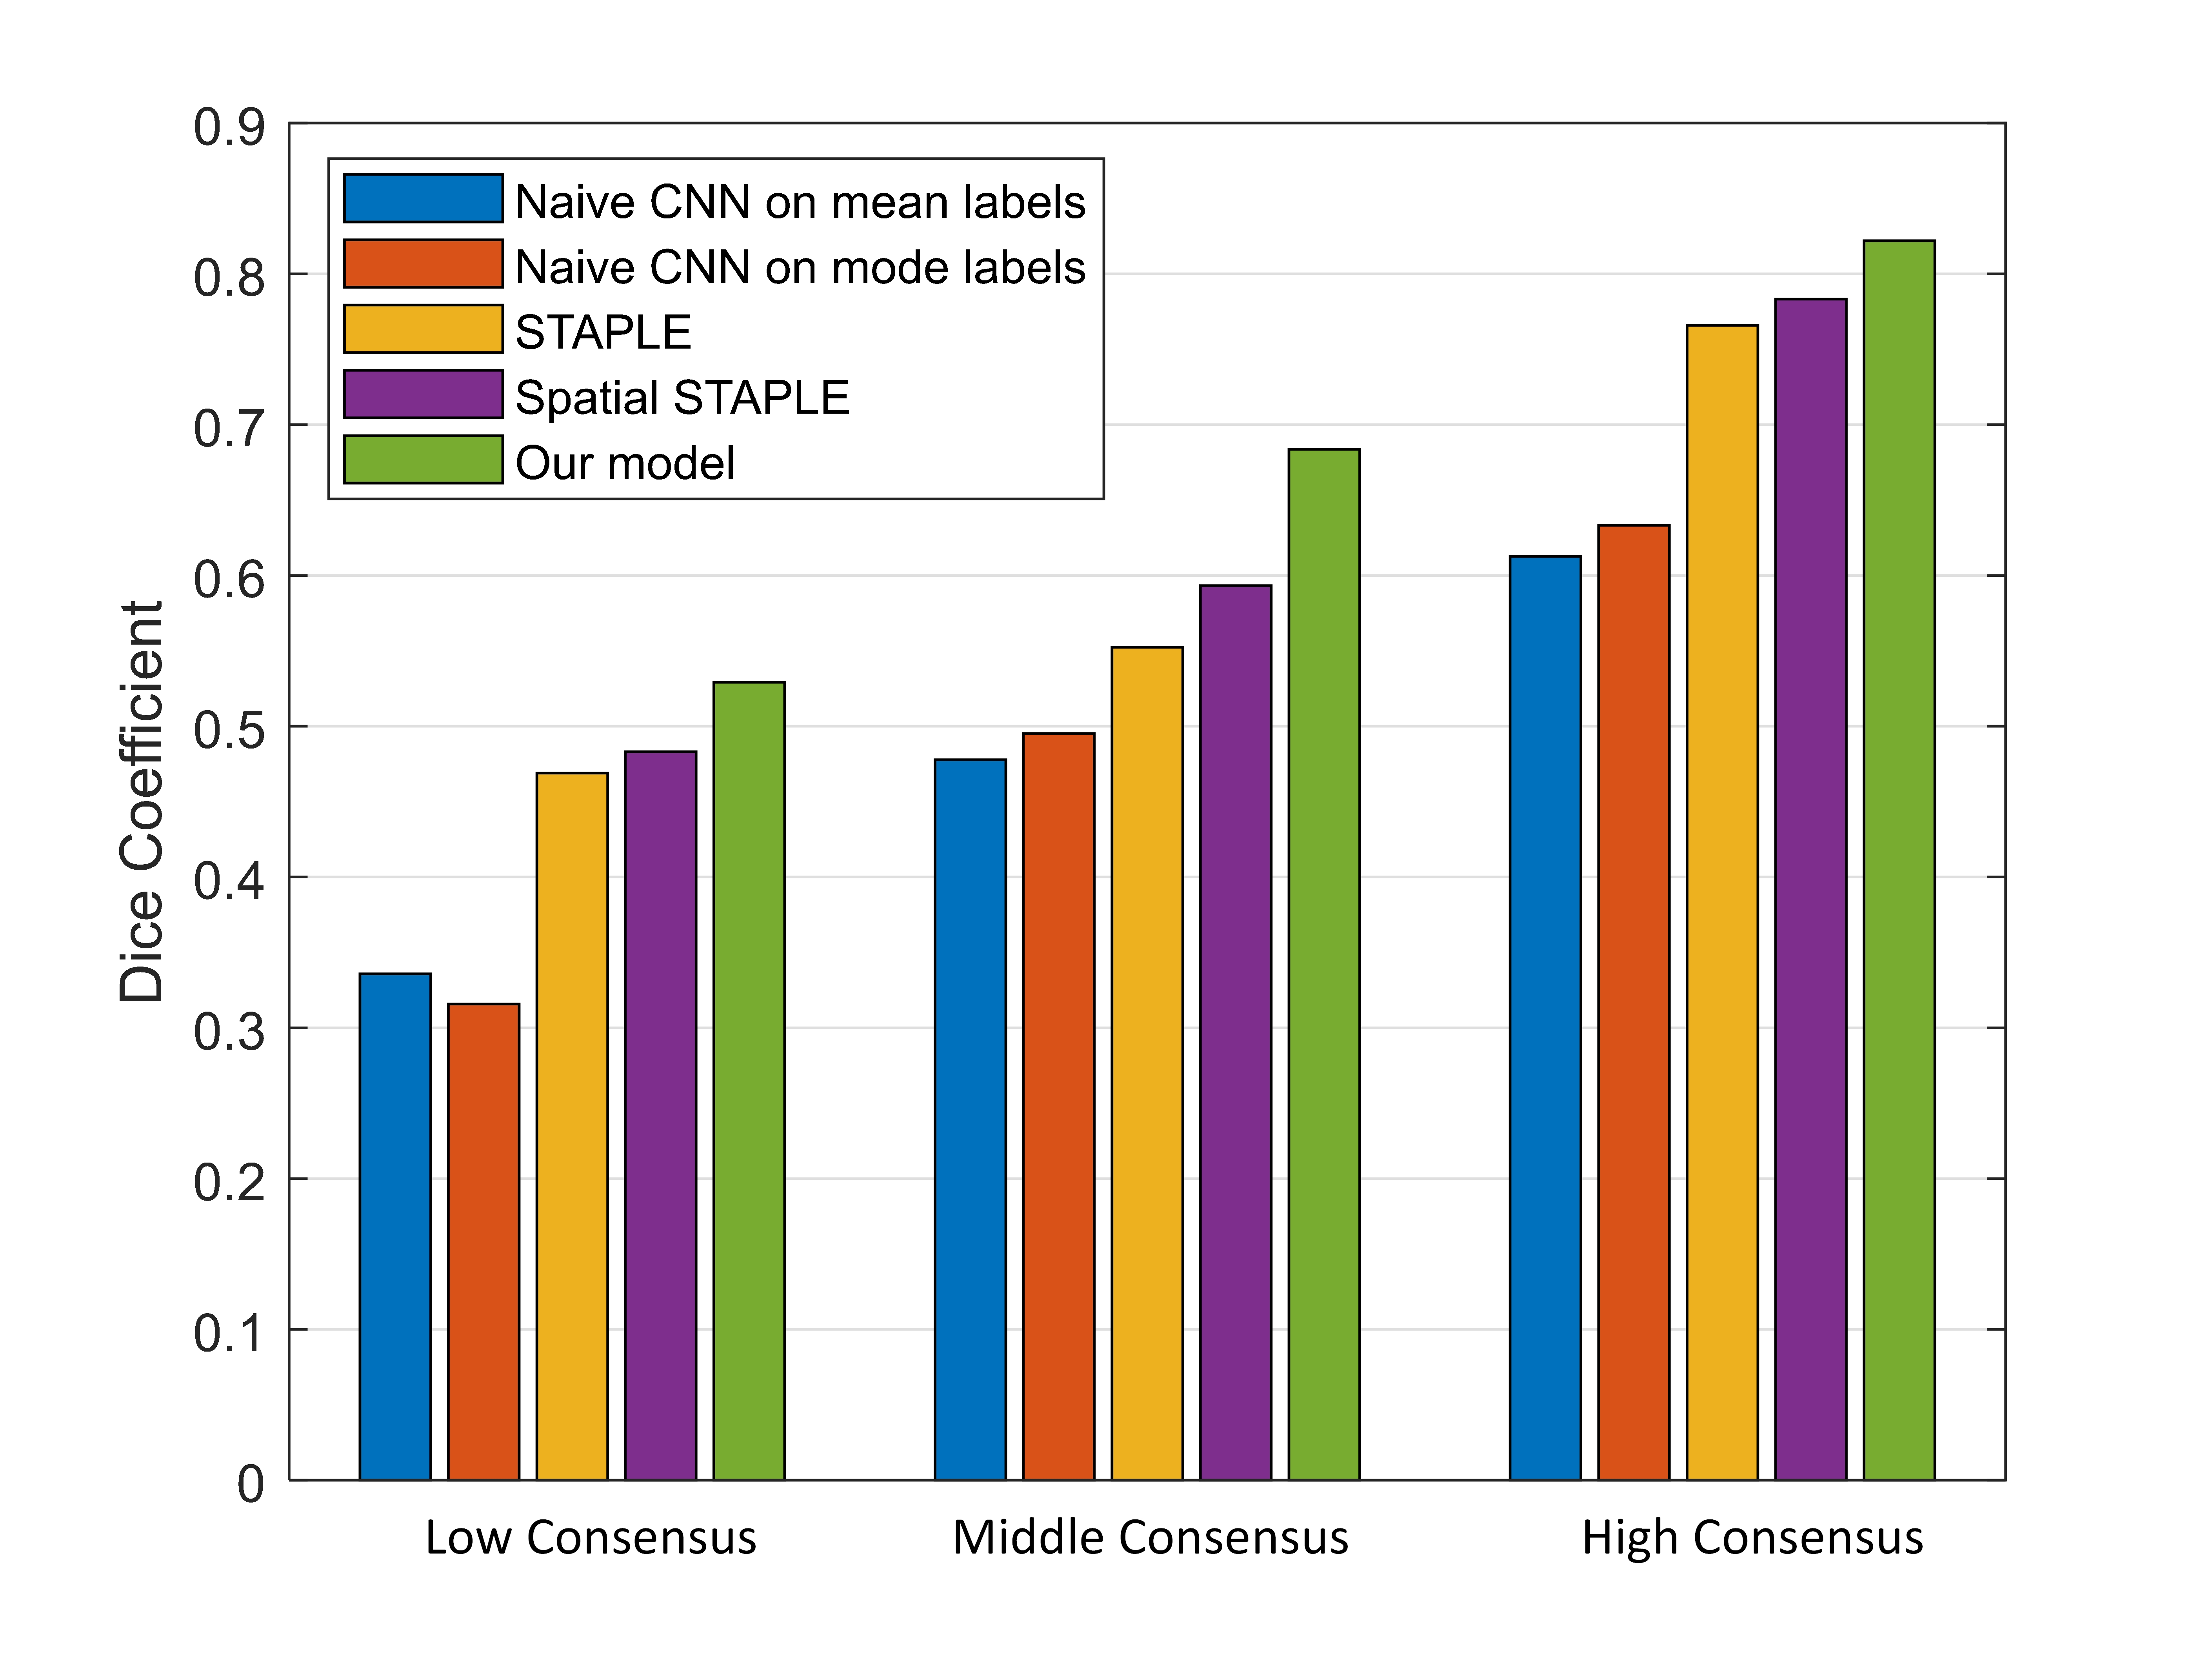
\includegraphics[scale=0.245]{chapter_8_neurips/picture19.jpg}
%        \caption{\footnotesize Segmentation performance on 3 different subgroups of the LIDC-IDRI dataset with varying levels of inter-reader agreement: 1) Low-consensus (30\% to 65\% IoU); 2) Middle consensus (65\% to 75\% IoU); 3) High consensus (75\% to 90\% IoU). Our method shows \textit{consistent} improvement over the baselines and the competing methods in all groups, showing its enhanced ability to segment challenging examples (i.e., low-consensus cases). }
%        \label{consensus dice}
%\end{figure}
%
%
%
%	\center
%	\begin{subfigure}[]{\linewidth}
%		\caption{Different classes of cardiac views}
%		\vspace{-3mm}	
%		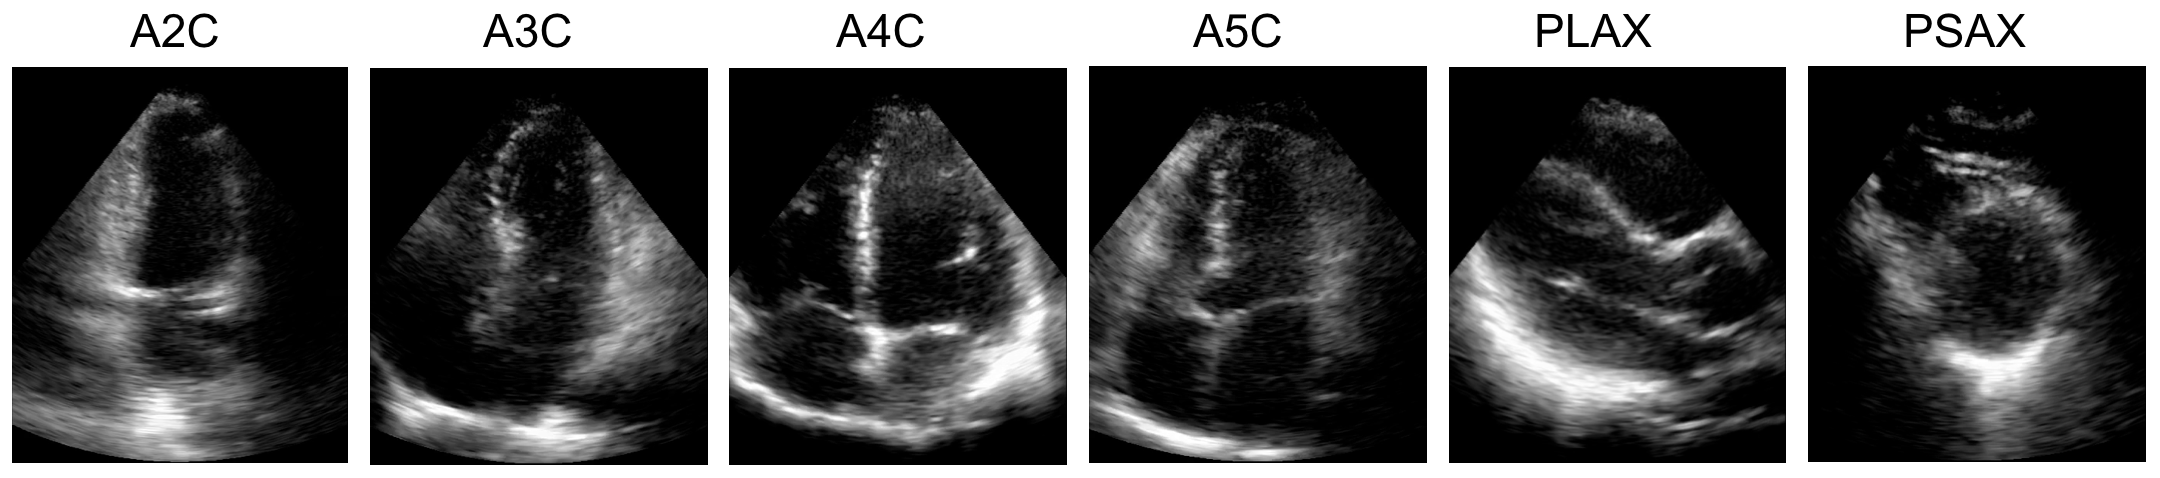
\includegraphics[width=\linewidth]{chapter_4/figures/figure_cardiac_views_02.png}
%	\end{subfigure}
%	\hspace{30mm}
%	\hfill
%	\begin{subfigure}[]{0.45\linewidth}
%		\vspace{3mm}
%		\caption{Skill estimation}
%		\vspace{-3mm}		
%		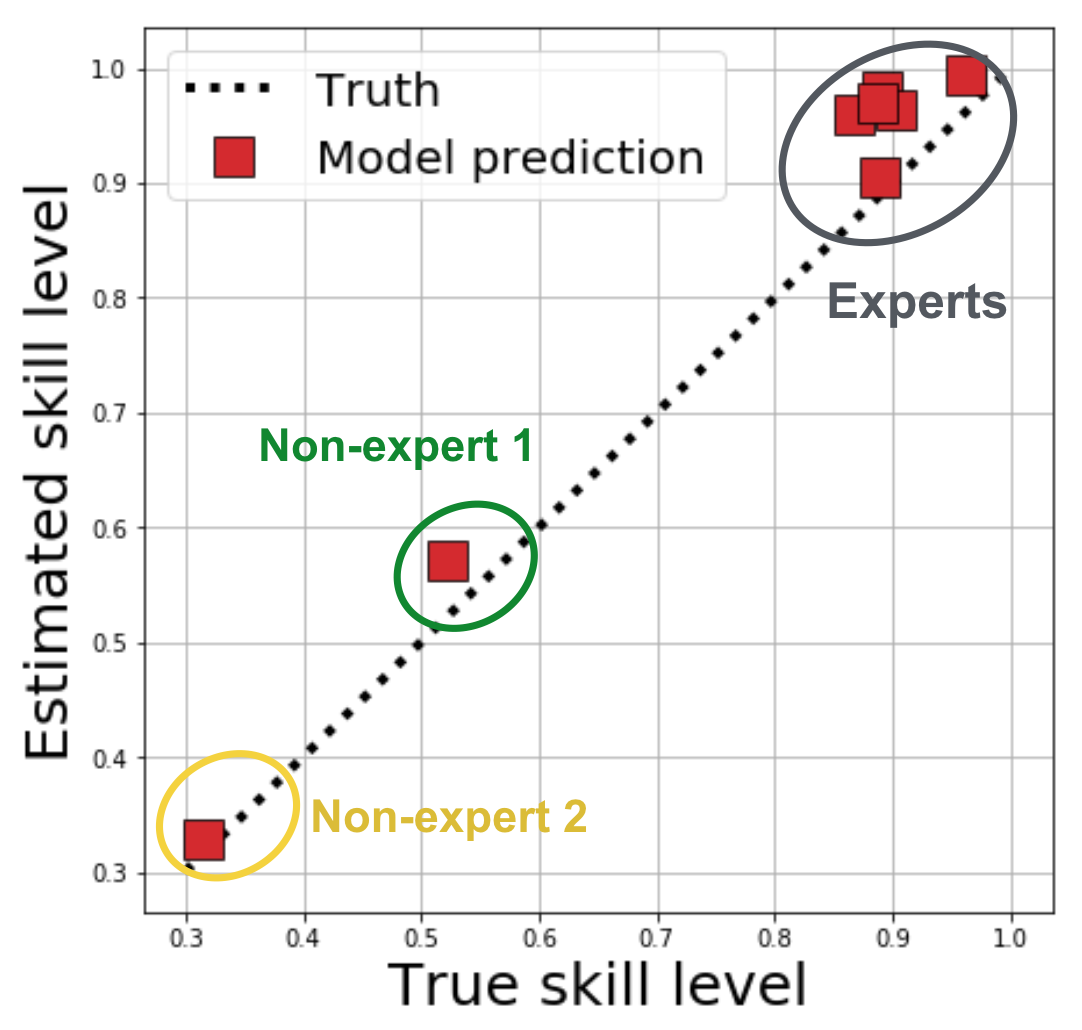
\includegraphics[width=0.9\linewidth]{chapter_4/figures/figure_real_us_annotator_clustering_03.png}
%	\end{subfigure}
%	\hspace{0mm}
%	\begin{subfigure}[]{0.75\linewidth}
%		\vspace{3mm}
%		\caption{Learned CMs}
%		\vspace{-3mm}
%		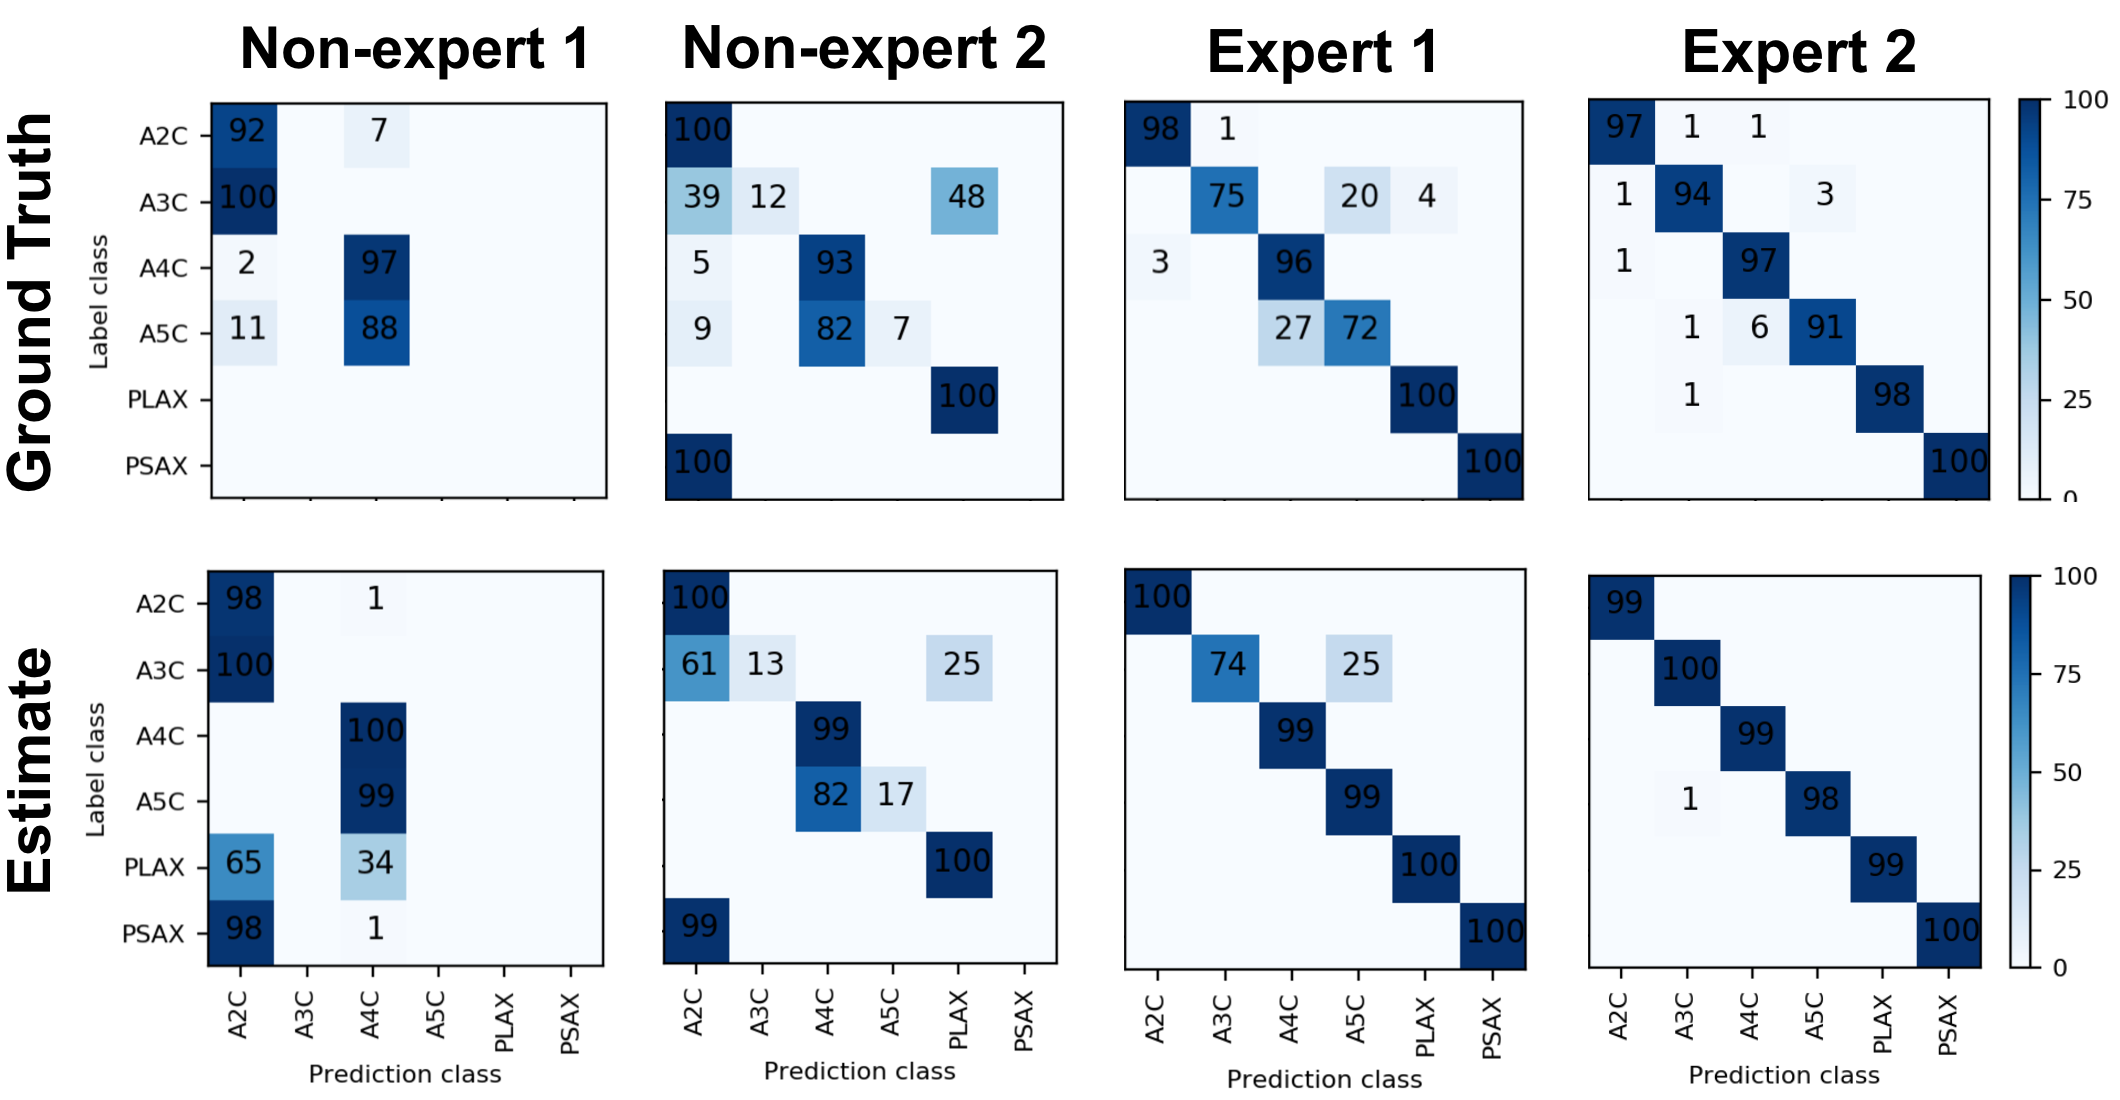
\includegraphics[width=\linewidth]{chapter_4/figures/figure_real_us_cms_visualization_02.png}
%	\end{subfigure}

Additionally, as shown in Table.\ref{ged_result}, our model consistently outperforms Probabilistic U-Net on generalized energy distance across the four test different datasets, indicating our method can better capture the inter-annotator variations than the baseline Probabilistic U-Net. This result shows that the information about which labels are acquired from whom is useful in modelling the variability in the observed segmentation labels. 

\begin{table}[t!]
	\center
	\footnotesize
	\begin{tabular}{@{}llllllllll}
		\hline
		 Models & MNIST & MS  & BraTS  & LIDC-IDRI  \\
		\hline	
		Probabilistic U-net \cite{kohl2018probabilistic}  & 1.46 $\pm$ 0.04 & 1.91 $\pm$ 0.03  & 3.23 $\pm$ 0.07  &  1.97 $\pm$ 0.03  \\
		Ours & \textbf{1.24 $\pm$ 0.02} & \textbf{1.67 $\pm$ 0.03}  & \textbf{3.14 $\pm$ 0.05}  &  \textbf{1.87 $\pm$ 0.04}  \\
		\hline
	\end{tabular}%
\caption{\footnotesize Comparison of Generalised Energy Distance (GED) on different datasets (mean $\pm$ standard deviation). The distance metric used here is the DICE score.}
\label{ged_result}
\end{table}



\section{Discussion and Conclusion}
We introduced the first supervised segmentation method for jointly estimating the spatial characteristics of labelling errors from multiple human annotators and the ground-truth label distribution. We demonstrated this method on real-world datasets with both synthetic and real-world annotations. Our method is capable of estimating individual annotators and thereby improving robustness against label noise. Experiments have shown our model achieves considerable improvement over the traditional label fusion approaches including averaging, the majority vote and the widely used STAPLE framework and its recent extensions, in terms of both segmentation accuracy and the quality of confusion matrix (CM) estimation.

In the future, we plan to accommodate meta-information of annotators (e.g., number of years of experience), and non-image data (e.g., genetics) that may influence the pattern of the underlying segmentation label such as lesion appearance, in our framework. We are also interested in assessing the utility of our approach in downstream applications. Of particular interest is the design of active data collection schemes where the segmentation model is used to select which samples to annotate (``active learning''), and the annotator models are used to decide which experts to label them (``active labelling'') \cite{yan2010modeling}. Another exciting avenue of applications is education of inexperienced annotators; the estimated spatial characteristics of segmentation mistakes provide further insights into their annotation behaviours, which they may benefit from in improving their annotation quality. 

%\subsection{Additional Qualitative Results on MNIST and MS Dataset}\label{Appendix MNIST and MS}
%%\ryu{(Ryu): lead each subsection with a succinct description of the extra results/details you are providing. For example, ``here we provide additional qualitative comparison of segmentation results on MNIST and MS datasets. ''. I would also have MNIST and MS dataset in two separate sections, but I understand if you already refer to them in the main text.  }
%
%Here we provide additional qualitative comparison of segmentation results and CM visualization results on MNIST and MS datasets. We examine the ability of our method to learn the CMs of annotators and the true label distribution on single label per image. Fig.~\ref{MNIST segmentation results for single label} and Fig.~\ref{MS segmentation results for sinle label} show the segmentation results on MNIST dataset on single label per image. Our model achieved a higher dice similarity coefficient than STAPLE and Spatial STAPLE, even prominently, our model outperformed STAPLE and Spatial STAPLE without or with trace norm, in terms of CM estimation. Fig.~\ref{CMs of MNIST - single label} and Fig.~\ref{CMs of MS - single label} illustrate our model on single label still can capture the patterns of mistakes.

%We compared the performance of our method against several baselines and the original STAPLE algorithm \cite{warfield2004simultaneous} and Spatial STAPLE \cite{asman2012formulating}. The first baseline is the naive CNN trained on the mean labels and the majority vote labels across the 5 annotators. \ryu{(ryu): do we not explain these baselines already in the main text. If we do already, I would just remove these descriptions of the baselines.}  The second baseline is the separate CNNs trained on 5 annotator labels and evaluate on their mean output. The “oracle” model is the idealistic scenario where CMs of the annotators are a priori known to the model while “annotators” indicate the average labeling accuracy of each annotator group. All the baselines and the annotator CNN, the segmentation CNN in our model are implemented with the NicMSlesions architecture described in \cite{VALVERDE2018101638}. We also evaluate on the validation set the effects of regularisation coefficient $\lambda \in \{0,0.001,0.01,0.1,0.4,0.7,0.9\}$ of the trace-norm in Eq. 4 on the accuracy of segmentation and CM estimation. Results are shown in Fig. \ref{Paramater lambda}. \ryu{(Ryu): why are you referring to Fig.~3 in the main text. It's better if we focused on describing the new contents we are adding here. } 

%\begin{figure}[H]
%    \centering
%    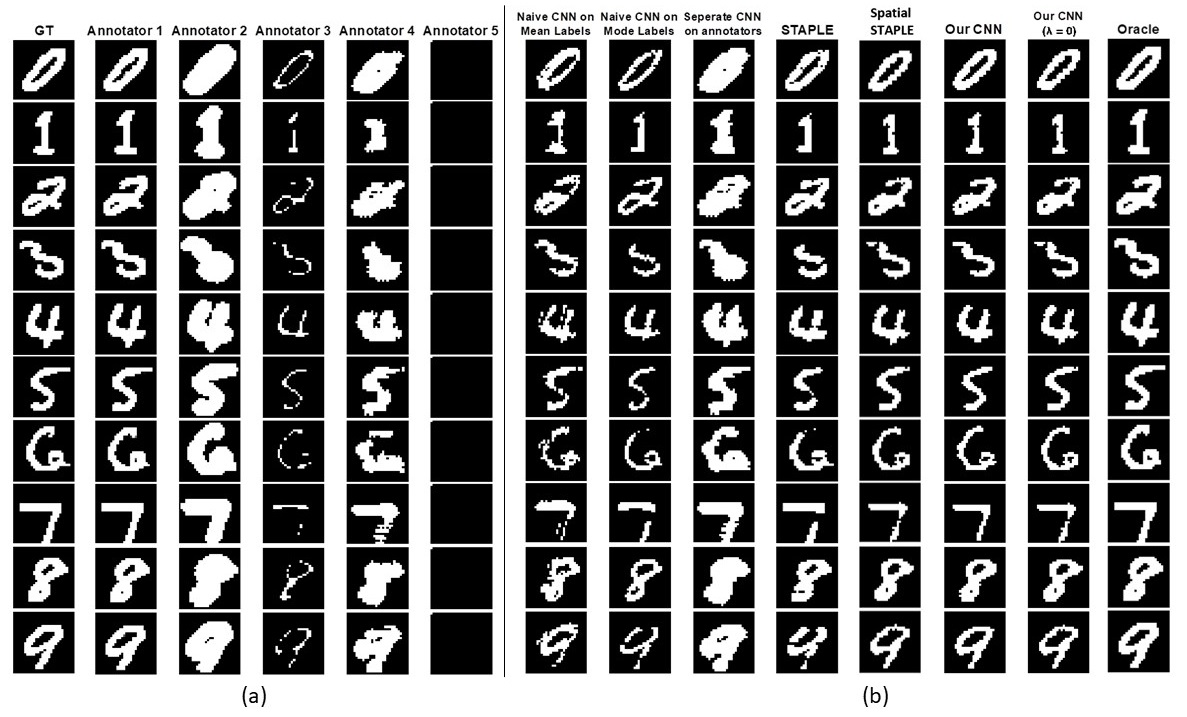
\includegraphics[width=\linewidth]{chapter_8_neurips/picture14.jpg}
%
%    \caption{\footnotesize Visualisation of segmentation labels on MNIST dataset for single label per image: (a) GT and simulated annotator's segmentations (Annotator 1 - 5); (b) the predictions from the supervised models.}
%    \label{MNIST segmentation results for single label}
%\end{figure}

%\begin{figure}[h]
%    \centering
%    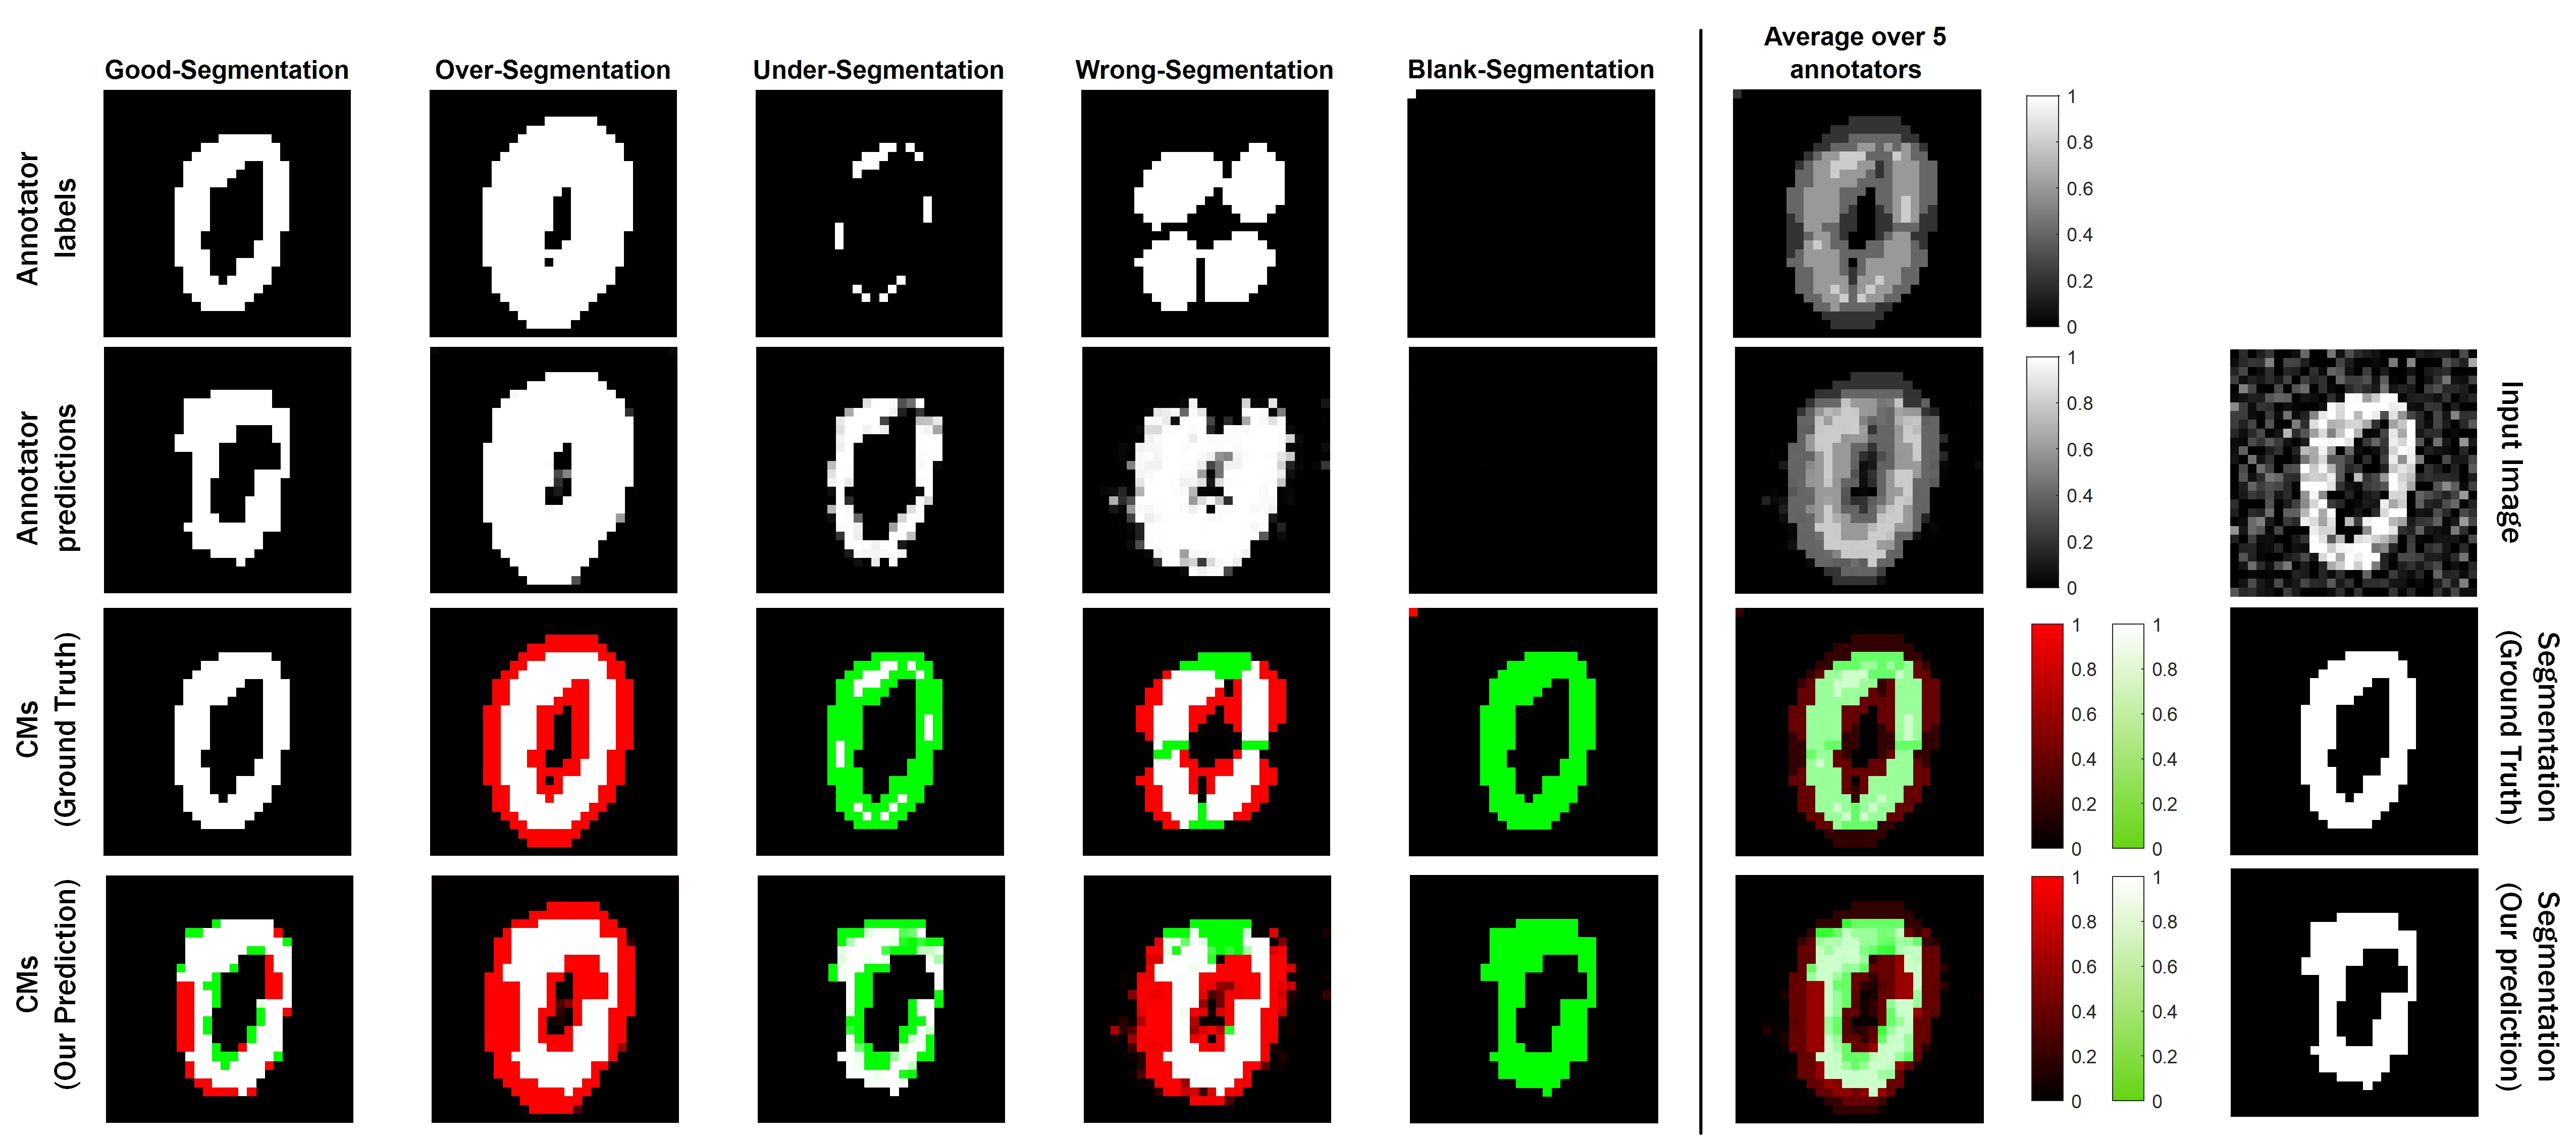
\includegraphics[width=\linewidth]{chapter_8_neurips/picture12.jpg}
%    %\addtocounter{figure}{+1}
%    \caption{\footnotesize Visualisation of estimated true labels and confusion matrices for single label per image on MNIST datasets (Best viewed in colour: white is the true positive, green is the false negative, red is the false positive and black is the true negative)}.%\ryu{We could also include more examples too. Perhaps, we can just convert 4 rows into only 2 rows (similar to Figure 2) e.g., put the third column next to the first, and the 4th next to the 2nd, and make the figure a lot smaller so you can include more examples.} }
%    \label{CMs of MNIST - single label}
%\end{figure}
%
%\begin{figure}[h]
%    \centering
%    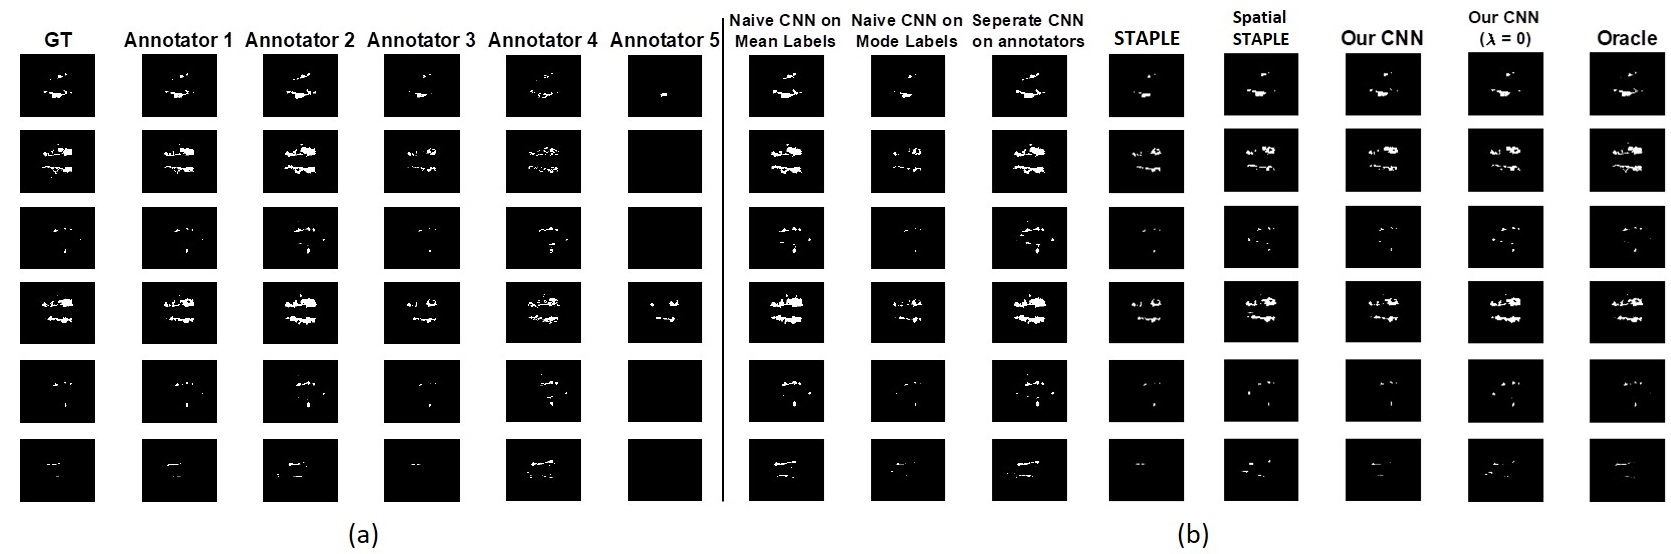
\includegraphics[width=\linewidth]{chapter_8_neurips/picture15.jpg}
%    \caption{\footnotesize Visualisation of segmentation labels on MS lesion dataset for single label per image: (a) GT and simulated annotator's segmentations (Annotator 1 - 5); (b) the predictions from the supervised models.}
%    \label{MS segmentation results for sinle label}
%\end{figure}

%\begin{figure}[!h]
%    \centering
%    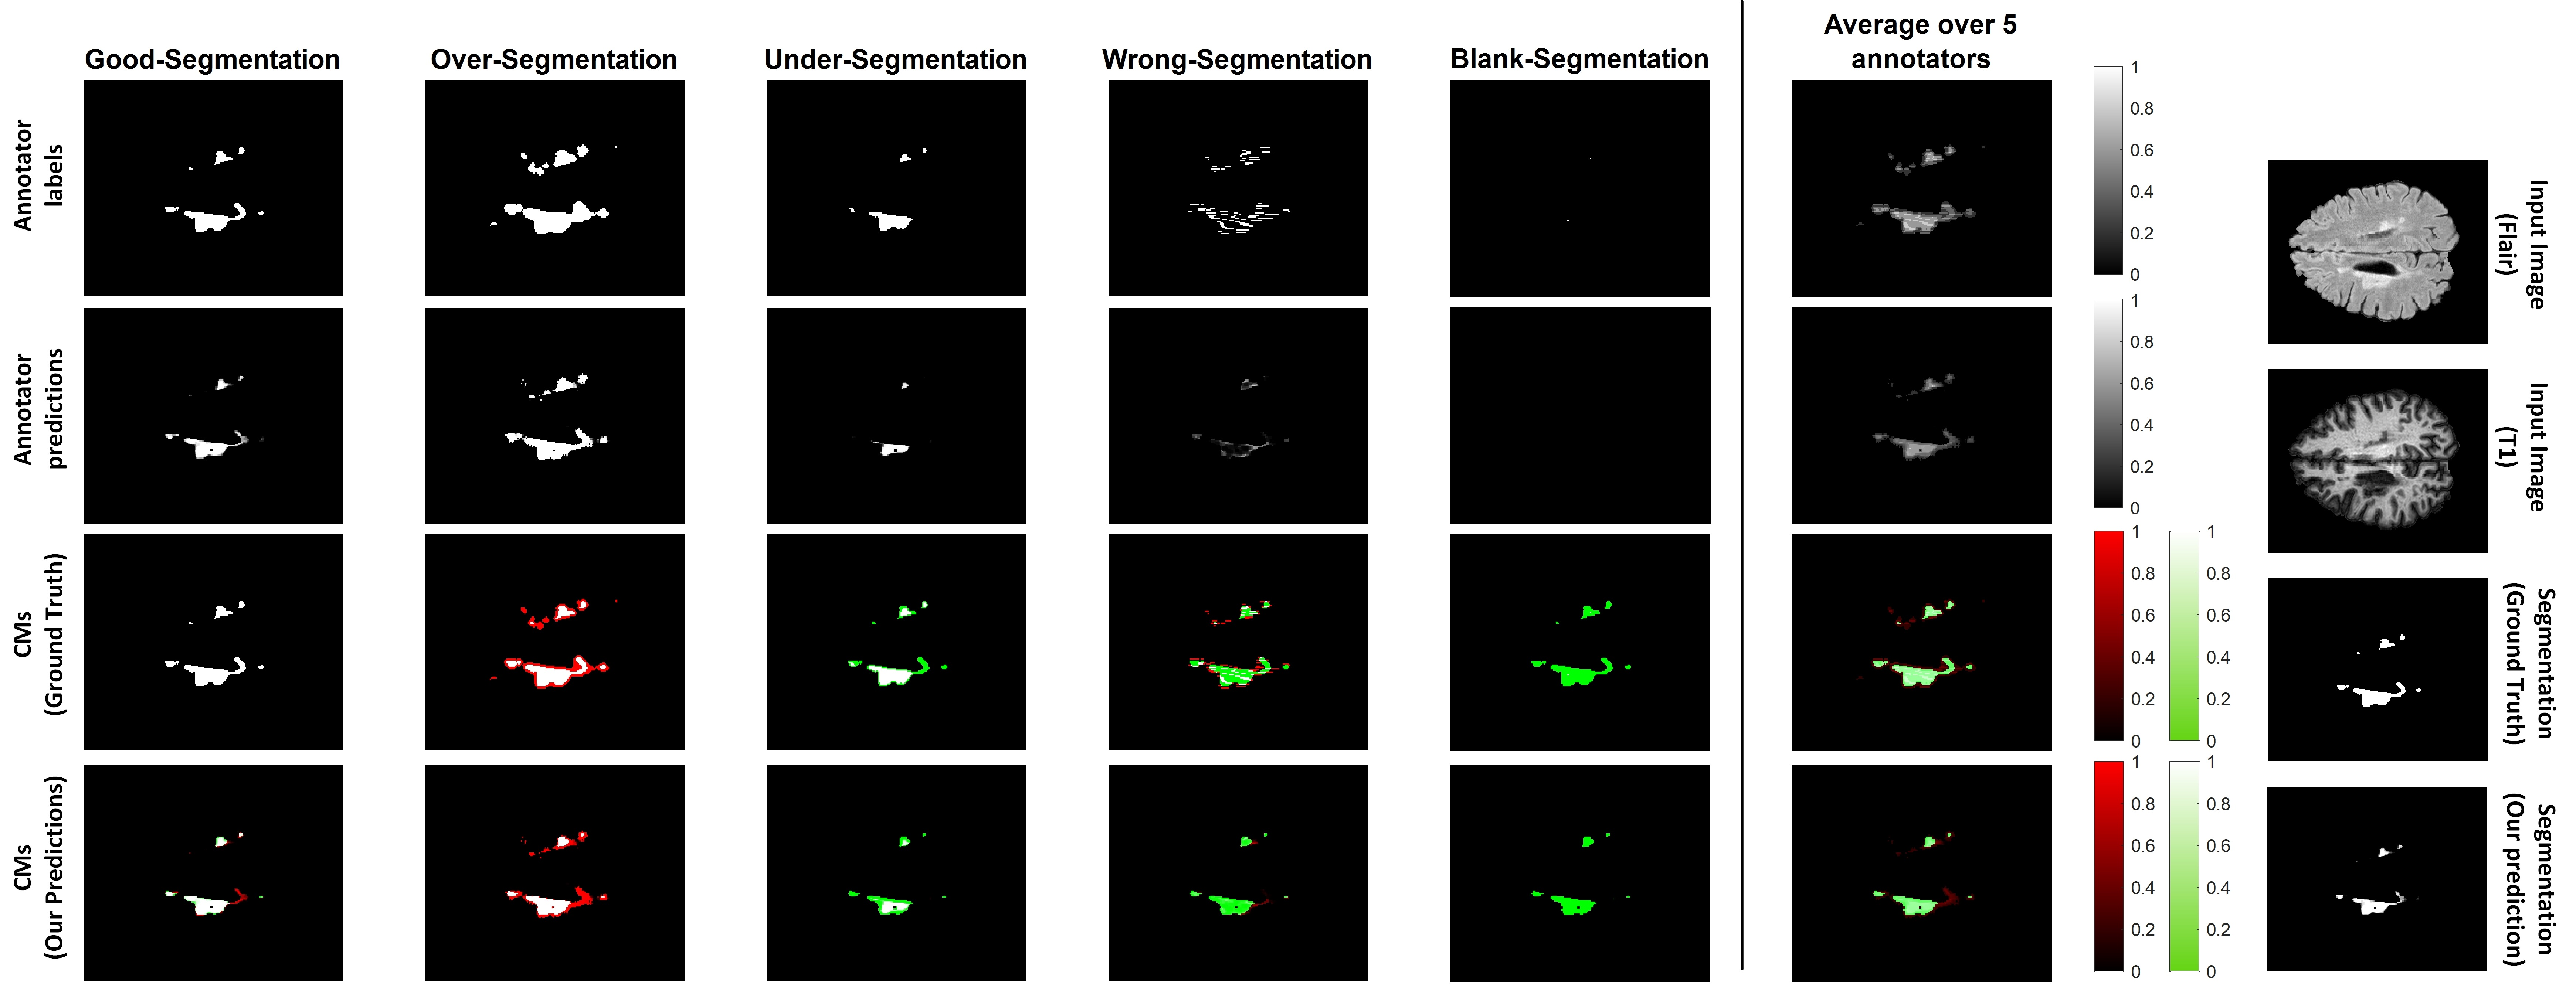
\includegraphics[width=\linewidth]{chapter_8_neurips/picture13.jpg}
%    %\addtocounter{figure}{+1}
%    \caption{\footnotesize Visualisation of estimated true labels and confusion matrices for single label per image on MS lesion datasets (Best viewed in colour: white is the true positive, green is the false negative, red is the false positive and black is the true negative). }
%    \label{CMs of MS - single label}
%\end{figure}



%\subsection{Quantitative and Extra Qualitative Results on BraTS and LIDC-IDRI}\label{Appendix Brats and LIDC-IDRI}
%\vspace{-2mm}
%%\ryu{(Ryu): we have not mentioned Fig.~\ref{LIDC segmentation}, \ref{consensus} and \ref{consensus dice} yet.} 
%
%
%%\ryu{(ryu): front-load with a short summary of what you provide in each subsection. Also, the titles of each subsections need to be more self-explanatory. The names of the datasets are not enough.} 
%
%%\ryu{Why don't we have two seprate sections? Currently it's not obvious what you are adding here. Just separate the contents into subsections to it's crystal clear what kinds of additional details or results you're adding here. The subsection title should  } 
%
%
%% \ryu{Here we provide results a, b, c, precluded from the main text. And point to figures.}
%
%Here we provide the quantitative comparison of our method and other baselines on BraTS and LIDC-IDRI datasets, which have been precluded from the main text due to the space limit (see Table.~\ref{denselabebrats} and Table. \ref{singlelabebrats}). We also provide additional qualitative examples (see Fig.~\ref{Brats results2},\ref{Brats results segmentation2}, \ref{LIDC segmentation}) on both datasets. Lastly, we compare the segmentation performance on 3 different subgroups of LIDC-IDRI with varying levels of inter-reader variability; Fig.~\ref{consensus dice} illustrates our method attains consistent improvement over the baselines in all cases, indicating its ability to segment more robustly even the hard examples where the experts in reality have disagreed to a large extent. 
%
%
%BraTS 2019 is a multi-class segmentation dataset, containing 259 cases with high grade (HG) and 76 cases with low grade (LG) glioma (a type of brain tumour). For each case, four MRI modalities are available, FLAIR, T1, T1-contrast and T2. The datasets are pre-processed by the organizers and co-registered to the same anatomical template, interpolated to the same resolution (1 $mm^3$) and skull-stripped. We used only high grade cases and centre cropped 2D images (192 $\times$ 192 pixels) and hold 1600 2D images for training, 300 images for validation, 500 images for testing, we apply Gaussian normalization on each case of each modality, to have zero-mean and unit variance. Fig. \ref{Brats results2} shows another tumor case in four different modality with different target label. We also present several example results on different methods in Fig.~\ref{Brats results segmentation2}. 
%
%To demonstrate the performance on a dataset with real-world annotations, we have also evaluated our model on LIDC-IDRI. The ``ground truth'' labels in the experiments are generated by aggregating the multiple labels via Spatial STAPLE\cite{asman2012formulating} as used in the curation of existing public datasets e.g., ISLES \cite{winzeck2018isles}, MSSeg \cite{commowick2018objective}, Gleason'19 \cite{gleason2019}. Fig.~\ref{LIDC segmentation} presents several examples of segmentation results from different methods. We also measure the inter-reader consensus level by computing the IoU of annotations, and compare in Fig.~\ref{consensus} the estimates from our model against the values meansured on the real annotations. Furthermore, we divide the test dataset into low consensus (30\% to 65\%), middle consensus (65\% to 75\%) and high consensus (75\% to 90\%) subgroups and compare the performance in Fig.~\ref{consensus dice}. Our method shows competitive ability to segment the challenging examples with low consensus values. Here we note that the consensus values in our test data range from 30\% to 90\%,, and compared the dice coefficient of our model with baselines. 

%The LIDC-IDRI dataset contains 1018 lung CT scans from 1010 lung patients with manual lesion segmentations from four experts. For each scan, 4 radiologists provided annotation masks for lesions that they independently detected and considered to be abnormal. For our experiments, we use the same method in \cite{kohl2018probabilistic} to pre-process all scans. We split the dataset at case-wise into a training (722 patients), validation (144 patients) and testing (144 patients). We then resampled the CT scans to $1 mm \times 1 mm$ in-plane resolution. We also centre cropped 2D images ($180 \times 180$ pixels) around lesion positions, in order to focus on the annotated lesions. The lesion positions are those where at least one of the experts segmented a lesion. We hold 5000 images in the training set, 1000 images in the validation set and 1000 images in the test set. 

%On both BraTS and LIDC-IDRI dataset, our proposed model consistenly achieves a higher dice similarity coefficient than STAPLE on both of the dense labels and single label scenarios (shown in Table.~\ref{denselabebrats} and Table. \ref{singlelabebrats}). In addition, our model (with trace) outperforms STAPLE in terms of CM estimation by a large margin at $14.4\%$ on BraTS. In Fig.~\ref{Brats results2}, we visualized the segmentation results on BraTS and the corresponding annotators' predictions. Fig.~\ref{Brats results segmentation2} presents four examples of the segmentation results and the corresponding annotators' predictions, as well as the baseline methods. As shown in both figures, our model successfully predicts the both the segmentation of lesions and the variations of each annotator in different cases. 


%
%\begin{figure}[h]
%    \vspace{-2mm}
%    \centering
%    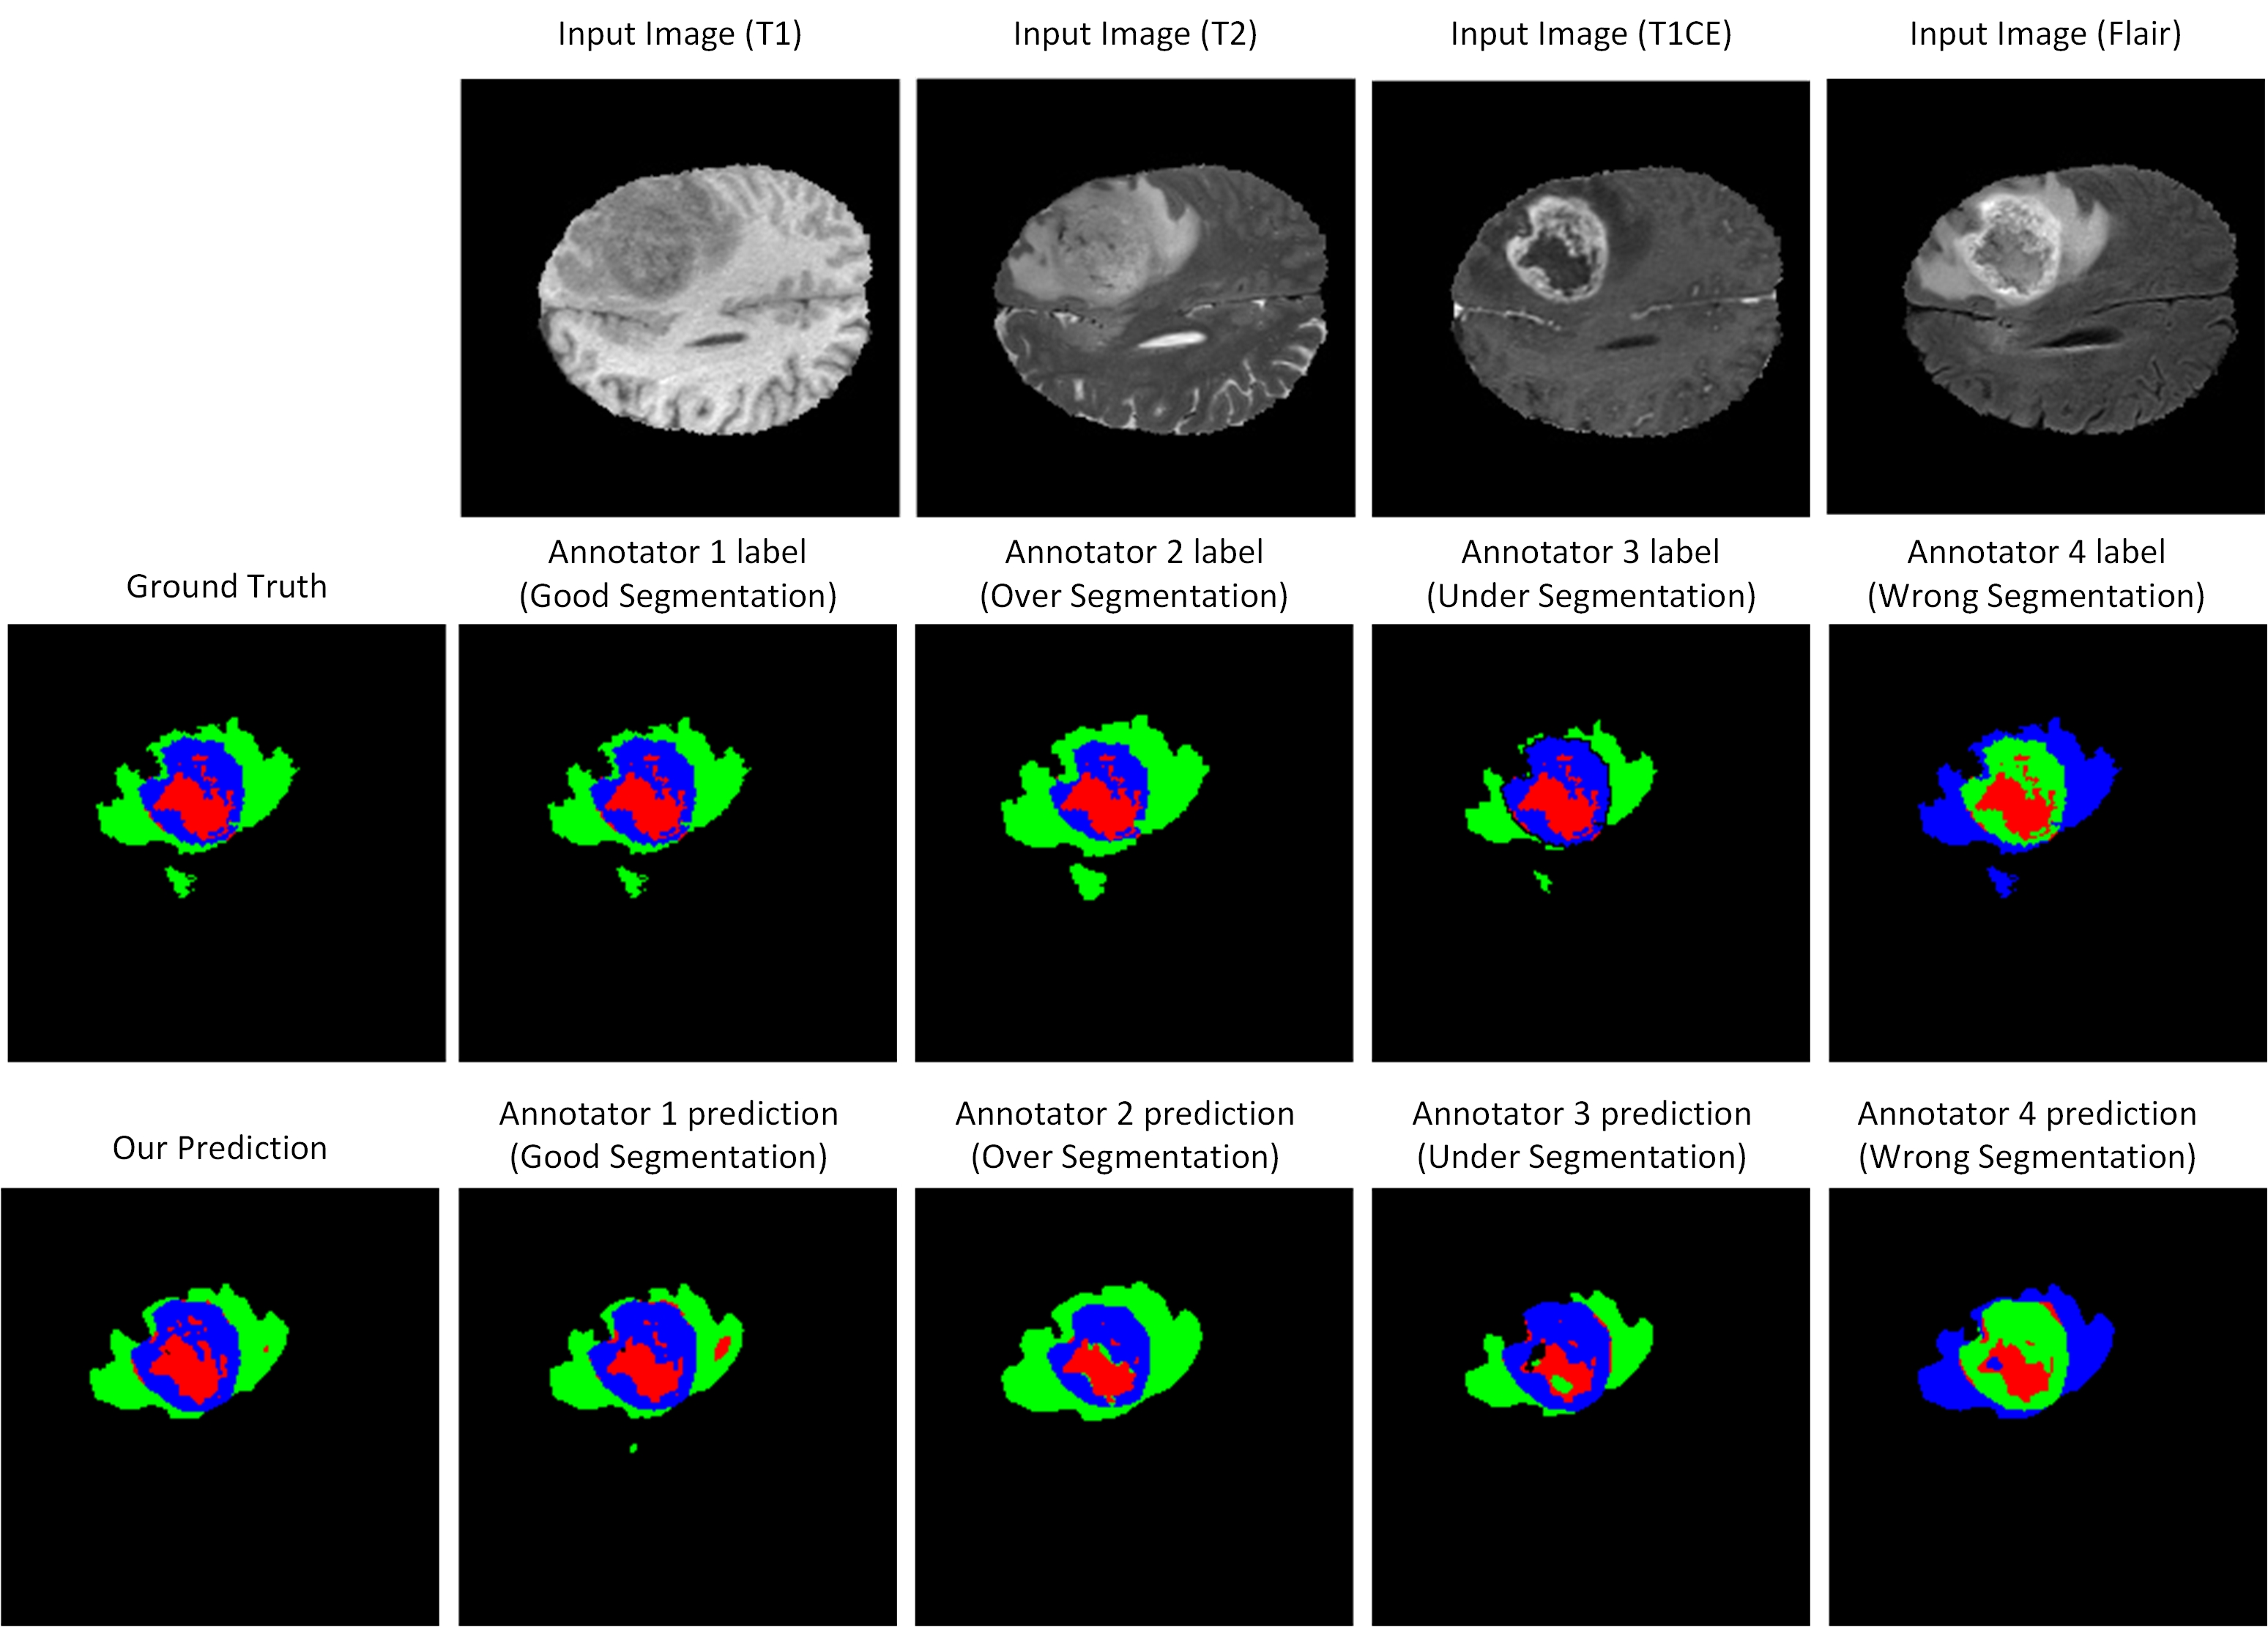
\includegraphics[scale=0.4]{chapter_8_neurips/picture9.jpg}
%    \caption{The final segmentation of our model on BraTS and each annotator network predictions visualization. (Best viewed in colour: the target label is green.)}
%    \label{Brats results2}
%    \vspace{-2mm}
%\end{figure}





